%% abtex2-modelo-trabalho-academico.tex, v-1.9.7 laurocesar
%% Copyright 2012-2018 by abnTeX2 group at http://www.abntex.net.br/ 
%%
%% This work may be distributed and/or modified under the
%% conditions of the LaTeX Project Public License, either version 1.3
%% of this license or (at your option) any later version.
%% The latest version of this license is in
%%   http://www.latex-project.org/lppl.txt
%% and version 1.3 or later is part of all distributions of LaTeX
%% version 2005/12/01 or later.
%%
%% This work has the LPPL maintenance status `maintained'.
%% 
%% The Current Maintainer of this work is the abnTeX2 team, led
%% by Lauro César Araujo. Further information are available on 
%% http://www.abntex.net.br/
%%
%% This work consists of the files abntex2-modelo-trabalho-academico.tex,
%% abntex2-modelo-include-comandos and abntex2-modelo-references.bib
%%
% ------------------------------------------------------------------------
% ------------------------------------------------------------------------
% abnTeX2: Modelo de Trabalho Academico (tese de doutorado, dissertacao de
% mestrado e trabalhos monograficos em geral) em conformidade com 
% ABNT NBR 14724:2011: Informacao e documentacao - Trabalhos academicos -
% Apresentacao
% ------------------------------------------------------------------------
% ------------------------------------------------------------------------
%%
%% Documento ajustado para PCS-EPUSP em 15/mar/2023 por Cintia Borges Margi
% ------------------------------------------------------------------------
%%
\documentclass[
	% -- opções da classe memoir --
	12pt,				% tamanho da fonte
	openright,			% capítulos começam em pág ímpar (insere página vazia caso preciso)
	twoside,			% para impressão em recto e verso. Oposto a oneside
	a4paper,			% tamanho do papel. 
	% -- opções da classe abntex2 --
	%chapter=TITLE,		% títulos de capítulos convertidos em letras maiúsculas
	%section=TITLE,		% títulos de seções convertidos em letras maiúsculas
	%subsection=TITLE,	% títulos de subseções convertidos em letras maiúsculas
	%subsubsection=TITLE,% títulos de subsubseções convertidos em letras maiúsculas
	% -- opções do pacote babel --
	english,			% idioma adicional para hifenização
	french,				% idioma adicional para hifenização
	spanish,			% idioma adicional para hifenização
	brazil				% o último idioma é o principal do documento
	]{abntex2}

% ---
% Pacotes básicos
% ---
\usepackage{lmodern}			% Usa a fonte Latin Modern
\usepackage[T1]{fontenc}		% Selecao de codigos de fonte.
\usepackage[utf8]{inputenc}		% Codificacao do documento (conversão automática dos acentos)
\usepackage{indentfirst}		% Indenta o primeiro parágrafo de cada seção.
\usepackage{color}				% Controle das cores
\usepackage{graphicx}			% Inclusão de gráficos
\usepackage{microtype} 			% para melhorias de justificação
% ---

% ---
% Pacotes adicionais
% ---
\usepackage{amsmath}			% Fórmulas matemáticas
\usepackage{amssymb}			% Símbolos matemáticos (\checkmark, \square, etc.)
\usepackage{booktabs}			% Tabelas com \toprule, \midrule, \bottomrule
\usepackage{listings}			% Blocos de código-fonte
\usepackage{xcolor}				% Cores para listings
% ---

% ---
% Configuração do listings
% ---
\lstset{
  basicstyle=\ttfamily\small,
  breaklines=true,
  breakatwhitespace=false,
  numbers=none,
  frame=single,
  tabsize=4,
  showstringspaces=false,
  keepspaces=true,
  commentstyle=\color{gray},
  keywordstyle=\color{black},
}
% ---

% ---
% Pacotes de citações
% ---
\usepackage[brazilian,hyperpageref]{backref}	 % Paginas com as citações na bibl
\usepackage[alf]{abntex2cite}	% Citações padrão ABNT

%% CBM: pacote para incluir a ficha catalográfica como pdf
\usepackage[final]{pdfpages}

% --- 
% CONFIGURAÇÕES DE PACOTES
% --- 

% ---
% Configurações do pacote backref
% Usado sem a opção hyperpageref de backref
\renewcommand{\backrefpagesname}{Citado na(s) página(s):~}
% Texto padrão antes do número das páginas
\renewcommand{\backref}{}
% Define os textos da citação
\renewcommand*{\backrefalt}[4]{
	\ifcase #1 %
		Nenhuma citação no texto.%
	\or
		Citado na página #2.%
	\else
		Citado #1 vezes nas páginas #2.%
	\fi}%
% ---

% ---
% Informações de dados para CAPA e FOLHA DE ROSTO
% ---
\titulo{GCC target for educational RISC-V processor}
\autor{Guilherme Stabach Salustiano}
\local{São Paulo, SP}
\data{2026}
\orientador{Prof. Dr. Bruno de Carvalho Albertini}
\instituicao{%
  Universidade de São Paulo -- USP
  \par
  Escola Politécnica
  \par
  Departamento de Engenharia de Computação e Sistemas Digitais (PCS)}
\tipotrabalho{Monografia de Conclusão de curso (Graduação)}
% O preambulo deve conter o tipo do trabalho, o objetivo,
% o nome da instituição e a área de concentração
\preambulo{Trabalho de conclusão de curso apresentado ao Departamento de Engenharia de Computação e Sistemas Digitais da Escola Politécnica da Universidade de São Paulo para obtenção do Título de Engenheiro.}
% ---


% ---
% Configurações de aparência do PDF final

% alterando o aspecto da cor azul
\definecolor{blue}{RGB}{41,5,195}

% informações do PDF
\makeatletter
\hypersetup{
     	%pagebackref=true,
		pdftitle={\@title}, 
		pdfauthor={\@author},
    	pdfsubject={\imprimirpreambulo},
	    pdfcreator={LaTeX with abnTeX2},
		pdfkeywords={abnt}{latex}{abntex}{abntex2}{trabalho acadêmico}, 
		colorlinks=true,       		% false: boxed links; true: colored links
    	linkcolor=blue,          	% color of internal links
    	citecolor=blue,        		% color of links to bibliography
    	filecolor=magenta,      		% color of file links
		urlcolor=blue,
		bookmarksdepth=4
}
\makeatother
% --- 

% ---
% Posiciona figuras e tabelas no topo da página quando adicionadas sozinhas
% em um página em branco. Ver https://github.com/abntex/abntex2/issues/170
\makeatletter
\setlength{\@fptop}{5pt} % Set distance from top of page to first float
\makeatother
% ---

% ---
% Possibilita criação de Quadros e Lista de quadros.
% Ver https://github.com/abntex/abntex2/issues/176
%
\newcommand{\quadroname}{Quadro}
\newcommand{\listofquadrosname}{Lista de quadros}

\newfloat[chapter]{quadro}{loq}{\quadroname}
\newlistof{listofquadros}{loq}{\listofquadrosname}
\newlistentry{quadro}{loq}{0}

% configurações para atender às regras da ABNT
\setfloatadjustment{quadro}{\centering}
\counterwithout{quadro}{chapter}
\renewcommand{\cftquadroname}{\quadroname\space} 
\renewcommand*{\cftquadroaftersnum}{\hfill--\hfill}

\setfloatlocations{quadro}{hbtp} % Ver https://github.com/abntex/abntex2/issues/176
% ---

% --- 
% Espaçamentos entre linhas e parágrafos 
% --- 

% O tamanho do parágrafo é dado por:
\setlength{\parindent}{1.3cm}

% Controle do espaçamento entre um parágrafo e outro:
\setlength{\parskip}{0.2cm}  % tente também \onelineskip

% ---
% compila o indice
% ---
\makeindex
% ---

% ----
% Início do documento
% ----
\begin{document}

% Seleciona o idioma do documento (conforme pacotes do babel)
\selectlanguage{english}
%\selectlanguage{brazil}

% Retira espaço extra obsoleto entre as frases.
\frenchspacing 

% ----------------------------------------------------------
% ELEMENTOS PRÉ-TEXTUAIS
% ----------------------------------------------------------
% \pretextual

% ---
% Capa
% ---
\imprimircapa
% ---

% ---
% Folha de rosto
% (o * indica que haverá a ficha bibliográfica)
% ---
\imprimirfolhaderosto*
% ---

% ---
% Inserir a ficha bibliografica
% ---

% Isto é um exemplo de Ficha Catalográfica, ou ``Dados internacionais de
% catalogação-na-publicação''. Você pode utilizar este modelo como referência. 
% Porém, provavelmente a biblioteca da sua universidade lhe fornecerá um PDF
% com a ficha catalográfica definitiva após a defesa do trabalho. Quando estiver
% com o documento, salve-o como PDF no diretório do seu projeto e substitua todo
% o conteúdo de implementação deste arquivo pelo comando abaixo:
%
%% TODO: utilizar a ficha catalográfica gerada em https://www.poli.usp.br/bibliotecas/servicos/catalogacao-na-publicacao
\begin{fichacatalografica}
    \includepdf{ficha.pdf}
\end{fichacatalografica}

% \begin{fichacatalografica}
% 	\sffamily
% 	\vspace*{\fill}					% Posição vertical
% 	\begin{center}					% Minipage Centralizado
% 	\fbox{\begin{minipage}[c][8cm]{13.5cm}		% Largura
% 	\small
% 	\imprimirautor
% 	%Sobrenome, Nome do autor
	
% 	\hspace{0.5cm} \imprimirtitulo  / \imprimirautor. --
% 	\imprimirlocal, \imprimirdata-
	
% 	\hspace{0.5cm} \thelastpage p. : il. (algumas color.) ; 30 cm.\\
	
% 	\hspace{0.5cm} \imprimirorientadorRotulo~\imprimirorientador\\
	
% 	\hspace{0.5cm}
% 	\parbox[t]{\textwidth}{\imprimirtipotrabalho~--~\imprimirinstituicao,
% 	\imprimirdata.}\\
	
% 	\hspace{0.5cm}
% 		1. Palavra-chave1.
% 		2. Palavra-chave2.
% 		3. Palavra-chave3.
% 		I. Orientador.
% 		II. Universidade xxx.
% 		III. Faculdade de xxx.
% 		IV. Título 			
% 	\end{minipage}}
% 	\end{center}
% \end{fichacatalografica}
% ---

% ---
% Inserir errata
% ---
% \begin{errata}
% Elemento opcional da \citeonline[4.2.1.2]{NBR14724:2011}. Exemplo:

% \vspace{\onelineskip}

% FERRIGNO, C. R. A. \textbf{Tratamento de neoplasias ósseas apendiculares com
% reimplantação de enxerto ósseo autólogo autoclavado associado ao plasma
% rico em plaquetas}: estudo crítico na cirurgia de preservação de membro em
% cães. 2011. 128 f. Tese (Livre-Docência) - Faculdade de Medicina Veterinária e
% Zootecnia, Universidade de São Paulo, São Paulo, 2011.

% \begin{table}[htb]
% \center
% \footnotesize
% \begin{tabular}{|p{1.4cm}|p{1cm}|p{3cm}|p{3cm}|}
%   \hline
%    \textbf{Folha} & \textbf{Linha}  & \textbf{Onde se lê}  & \textbf{Leia-se}  \\
%     \hline
%     1 & 10 & auto-conclavo & autoconclavo\\
%    \hline
% \end{tabular}
% \end{table}

% \end{errata}
% ---

% ---
% Inserir folha de aprovação
% ---

% Isto é um exemplo de Folha de aprovação, elemento obrigatório da NBR
% 14724/2011 (seção 4.2.1.3). Você pode utilizar este modelo até a aprovação
% do trabalho. Após isso, substitua todo o conteúdo deste arquivo por uma
% imagem da página assinada pela banca com o comando abaixo:
%
% \begin{folhadeaprovacao}
% \includepdf{folhadeaprovacao_final.pdf}
% \end{folhadeaprovacao}
%
% \begin{folhadeaprovacao}

%   \begin{center}
%     {\ABNTEXchapterfont\large\imprimirautor}

%     \vspace*{\fill}\vspace*{\fill}
%     \begin{center}
%       \ABNTEXchapterfont\bfseries\Large\imprimirtitulo
%     \end{center}
%     \vspace*{\fill}
    
%     \hspace{.45\textwidth}
%     \begin{minipage}{.5\textwidth}
%         \imprimirpreambulo
%     \end{minipage}%
%     \vspace*{\fill}
%    \end{center}
        
%    Trabalho aprovado. \imprimirlocal, 24 de novembro de 2012:

%    \assinatura{\textbf{\imprimirorientador} \\ Orientador} 
%    \assinatura{\textbf{Professor} \\ Convidado 1}
%    \assinatura{\textbf{Professor} \\ Convidado 2}
%    %\assinatura{\textbf{Professor} \\ Convidado 3}
%    %\assinatura{\textbf{Professor} \\ Convidado 4}
      
%    \begin{center}
%     \vspace*{0.5cm}
%     {\large\imprimirlocal}
%     \par
%     {\large\imprimirdata}
%     \vspace*{1cm}
%   \end{center}
  
% \end{folhadeaprovacao}
% ---

% ---
% Dedicatória
% ---
\begin{dedicatoria}
   \vspace*{\fill}
   \centering
   \noindent
   \textit{Para que serve tantos codigos, se a vida nao é programada\\
   e as melhores coisas não tem logica.} \vspace*{\fill}
\end{dedicatoria}
% ---

% ---
% Agradecimentos
% ---
\begin{agradecimentos}
The main acknowledgements are directed to \ldots

% TODO: fill acknowledgements
\end{agradecimentos}
% ---

% ---
% Epígrafe
% ---
% \begin{epigrafe}
%     \vspace*{\fill}
% 	\begin{flushright}
% 		\textit{...}
% 	\end{flushright}
% \end{epigrafe}
% ---

% ---
% RESUMOS
% ---

% resumo em português
\setlength{\absparsep}{18pt} % ajusta o espaçamento dos parágrafos do resumo
\begin{resumo}
% TODO: escrever o resumo em português

 \textbf{Palavras-chave}: GCC. RISC-V. Compilador. Processador educacional.
\end{resumo}

% resumo em inglês
\begin{resumo}[Abstract]
 \begin{otherlanguage*}{english}
   This is the english abstract.

   \vspace{\onelineskip}

   \noindent
   \textbf{Keywords}: GCC. RISC-V. Compiler. Educational processor.
 \end{otherlanguage*}
\end{resumo}

% % resumo em francês 
% \begin{resumo}[Résumé]
%  \begin{otherlanguage*}{french}
%     Il s'agit d'un résumé en français.
 
%    \textbf{Mots-clés}: latex. abntex. publication de textes.
%  \end{otherlanguage*}
% \end{resumo}

% % resumo em espanhol
% \begin{resumo}[Resumen]
%  \begin{otherlanguage*}{spanish}
%    Este es el resumen en español.
  
%    \textbf{Palabras clave}: latex. abntex. publicación de textos.
%  \end{otherlanguage*}
% \end{resumo}
% ---

% ---
% inserir lista de ilustrações
% ---
\pdfbookmark[0]{\listfigurename}{lof}
\listoffigures*
\cleardoublepage
% ---

% ---
% inserir lista de quadros
% ---
\pdfbookmark[0]{\listofquadrosname}{loq}
\listofquadros*
\cleardoublepage
% ---

% ---
% inserir lista de tabelas
% ---
\pdfbookmark[0]{\listtablename}{lot}
\listoftables*
\cleardoublepage
% ---

% ---
% inserir lista de abreviaturas e siglas
% ---
\begin{siglas}
  \item[ABI] \textit{Application Binary Interface}
  \item[AMO] \textit{Atomic Memory Operation}
  \item[CSR] \textit{Control and Status Register}
  \item[ELF] \textit{Executable and Linkable Format}
  \item[GCC] \textit{GNU Compiler Collection}
  \item[GNU] \textit{GNU's Not Unix}
  \item[ISA] \textit{Instruction Set Architecture}
  \item[PIC] \textit{Position-Independent Code}
  \item[RISC] \textit{Reduced Instruction Set Computer}
  \item[RTL] \textit{Register Transfer Language}
  \item[RV32I] RISC-V, integers, 32 bits
  \item[RV64I] RISC-V, integers, 64 bits
\end{siglas}
% ---

% ---
% inserir o sumario
% ---
\pdfbookmark[0]{\contentsname}{toc}
\tableofcontents*
\cleardoublepage
% ---


% ----------------------------------------------------------
% ELEMENTOS TEXTUAIS
% ----------------------------------------------------------
\textual

% Chapter 1. Introduction
\chapter{Introduction} \label{cap:intro}

\section{Motivation}

\textit{Computer Organization and Design: RISC-V Edition} by Patterson and Hennessy \cite{patterson2020}
is one of the most widely adopted references in undergraduate computer architecture courses worldwide.
At the University of São Paulo's Escola Politécnica, the course \textit{PCS3225 --- Digital Systems 2}
uses this textbook as its primary reference. Students follow its progression step by step, implementing
a simplified RISC-V processor in Verilog from book reference.

The simplified single-cycle processor introduced in Chapter 4.4 of the book, \textit{A Simple
Implementation Scheme}, supports only eight instructions: \texttt{lw}, \texttt{sw}, \texttt{beq},
\texttt{add}, \texttt{addi}, \texttt{sub}, \texttt{and}, and \texttt{or}. This restriction is
deliberate and pedagogically motivated, it isolates the essential datapath and control concepts before
more complex features are introduced. A subsequent homework assignment extends the processor with
\texttt{lui} and \texttt{jalr}, enabling function calls. Both implementations are partial subsets of
the RV32I base ISA \cite{riscv-spec}.

This restriction creates a practical barrier. The standard RISC-V GCC toolchain
(\texttt{riscv32-unknown-elf-gcc}) targets the full RV32I base ISA \cite{riscv-spec}, which includes
shift instructions, byte and halfword memory operations, multiple branch variants, and PC-relative
addressing. Any C program compiled with this toolchain will emit instructions that the student-built
processor cannot execute.

As a result, students are limited to running hand-written assembly or small programs provided by the
professor. They cannot compile and run arbitrary C code on the processor they designed and built. This
prevents them from connecting the hardware they implement to the software abstractions they use daily,
and forecloses the pedagogical opportunity of observing how a compiler translates and optimizes C code
into the primitive instructions their processor supports.

\section{Objective}

This work develops eight progressive GCC compiler targets for the simplified RISC-V processors
described in the Hennessy and Patterson textbook, enabling students of the PCS3225 course at USP to
compile and run C programs on the processors they build in Verilog.

The specific objectives are:

\begin{enumerate}
  \item Define a minimal GCC target (\texttt{rvsc0}) matching the eight-instruction single-cycle
        processor described in Chapter 4.4 of the textbook, synthesizing all operations not natively
        supported by that processor.
  \item Define a target (\texttt{rvsc1}) matching the course homework processor, \texttt{rvsc0}
        extended with \texttt{lui} and \texttt{jalr}, as the minimum instruction set capable of
        supporting the full C calling convention with synthesis.
  \item Define six additional progressive targets (\texttt{rvsc2} through \texttt{rvsc7}),
        incrementally extending the supported instruction set from bare RV32I through RV64IMAFD,
        for students who wish to continue developing their processor beyond the course scope.
  \item Synthesize every instruction not natively supported by a given target as an equivalent
        sequence of instructions that the target does support.
\end{enumerate}

\section{Rationale}

To the best of the author's knowledge, no prior work addresses C compilation for intentionally
restricted pedagogical RISC-V subsets. GCC's machine description framework \cite{gcc-internals} makes
it possible to define a backend that synthesizes missing instructions transparently from the primitives
the hardware does support. Applying this mechanism to pedagogical ISAs that deliberately omit standard
instructions appears to be novel.

The ability to run a self-written C program on a processor the student designed and built closes a
pedagogical loop that rarely closes in undergraduate education. Most courses treat hardware and software
as adjacent subjects that never directly intersect. This work creates a complete vertical slice from C
source to register-level execution on student hardware. Students can compile a function, inspect the
output, and observe concretely how the compiler synthesizes a shift operation from repeated additions,
or a signed comparison from subtraction and bit manipulation, making the cost of each ISA restriction
tangible rather than abstract.

Furthermore, students interact with GCC, the dominant open-source compiler for embedded and systems
software, rather than a pedagogical toy. The flags, ABI conventions, ELF output, and linker scripts
they encounter are identical to those used in professional and research settings, giving the exercise
relevance beyond the course itself.

\section{Document Organization}

The remainder of this monograph is organized as follows.
Chapter~\ref{cap:related-work} surveys related work, in instruction synthesis for embedded compiler
backends and in tools for instruction-set-level computing education.
Chapter~\ref{cap:background} presents the conceptual background: the RISC-V instruction set, the
single-cycle datapath of the Hennessy-Patterson educational processor, the C calling convention the
targets must honour, and the structure of a GCC backend.
Chapter~\ref{cap:method} describes the development method, including the derivation cycle applied to
each synthesized instruction and the validation approach.
Chapter~\ref{cap:requirements} specifies the requirements for each of the eight targets, defining
the allowed instruction sets and the synthesis obligations imposed on the compiler.
Chapter~\ref{cap:development} details the implementation: a correctness argument and an instruction
sequence for every synthesis, the machine-description and per-target configuration that make them
transparent to the programmer, and the limitations that remain.
Chapter~\ref{cap:results} reports the three test layers, quantifies the static and dynamic cost of
synthesis on the Embench-IoT suite, and discusses what the measurements do and do not establish.
Chapter~\ref{cap:conclusion} presents the conclusions, contributions, and directions for future work.
The appendices collect the compiler output that the synthesis sections refer to, including a worked
compilation example across rvsc0, rvsc1 and rvsc2.


% Chapter 2. Related Work + Conceptual Background
% ---------------------------------------------------------------
% Chapter 2: Related Work
% ---------------------------------------------------------------
\chapter{Related Work} \label{cap:related-work}

Two bodies of work bear on this project: GCC's established mechanisms for synthesizing
hardware-absent operations, applied in the embedded domain for decades; and pedagogical tools for
instruction-set-level computing education.

\section{Instruction Synthesis in Compiler Backends}

GCC has long supported targets whose processors lack hardware instructions for certain operations. The
canonical example is soft-float: on a target without a floating-point unit, the compiler replaces every
floating-point operation by a call to a library routine that implements IEEE~754 arithmetic with
integer instructions, with no change required from the programmer \cite{gcc-internals}. Two properties
of that substitution matter here, and both reappear in this work. The first is that the replacement is
a body of carefully validated software arithmetic rather than an incidental expansion: the Berkeley
SoftFloat package \cite{softfloat} is the reference implementation of that kind, and is the arithmetic
model inside the Spike simulator against which this work validates its own output. The second is that
the substitution is an ABI contract rather than a private decision of one compiler. The Arm run-time
ABI \cite{arm-rtabi} names each helper routine and fixes its calling convention, so that soft-float
objects produced by different compilers interoperate; GCC documents the equivalent set for its own
targets as part of libgcc \cite{gcc-internals}, where the same mechanism extends to integer operations,
with routines such as \texttt{\_\_mulsi3} and \texttt{\_\_ashlsi3} existing precisely because some
targets have neither a multiplier nor a multi-bit shift.

Those integer cases are the closest existing precedent for this work. The MSP430 has no multi-bit shift
instruction: a shift by more than one position is either a repeated single-bit operation or a call to
one of the runtime helpers the MSP430 embedded ABI defines for the purpose, among them
\texttt{\_\_mspabi\_slli\_n}, \texttt{\_\_mspabi\_srli\_n} and their long and arithmetic variants
\cite{msp430-eabi,msp430-ug}. The AVR is more restricted still. Its shift and rotate instructions move
exactly one bit \cite{avr-isa}, so GCC's AVR backend emits a straight-line run of \texttt{lsl} or
\texttt{lsr} for a small constant count and a counted loop for a variable one --- the same two
constructions this work derives for rvsc1 in Section~\ref{sec:sc1-sll}, reached independently from the
same constraint. Hardware multiplication is likewise present only on the enhanced AVR cores; on the
classic and reduced-tiny devices \texttt{\_\_mulqi3} and \texttt{\_\_mulhi3} are shift-and-add routines
in libgcc \cite{avr-isa}. \citeonline{hauser2020} quantify what such substitutions cost on embedded
RISC-V targets, showing that backend choices have a measurable impact on code size.

In all these cases the programmer writes standard C and the compiler silently emits the replacement
sequence, at the cost of additional instructions and a correspondingly larger binary. What
distinguishes the present work is the proportion of the instruction set involved. A soft-float or
multiplier-less target is missing a category of operations; the sc0 and sc1 targets are missing nearly
everything, and must synthesize shifts, exclusive or, ordered comparisons, all conditional branches
other than \texttt{beq}, every sub-word load and store, and --- on sc0 --- the loading of a large
constant, out of eight or ten remaining instructions.

\section{Pedagogical Instruction-Set Tools}

A distinct body of work provides tools for computer architecture education at the assembly level. Venus
\cite{venus}, RARS \cite{rars}, and MARS \cite{mars} are simulators that accept programs written
directly in assembly and execute them step by step. None of them performs C compilation; the programmer
works at the assembly level from the outset.

BRISC-V \cite{brisc-v} provides an open-source parameterised RISC-V processor family for computer
architecture education together with a standard GCC toolchain. The toolchain targets the full RV32I
instruction set, with no mechanism to restrict the compiler to a hardware-defined subset.

This work sits at the intersection of the two lines: it brings the instruction synthesis approach
from the embedded compiler domain, applied to a far smaller instruction subset,
into the pedagogical setting of the Hennessy-Patterson processor \cite{patterson2020},
enabling students to write C programs that run correctly on a processor with a deliberately minimal
instruction set --- one they built themselves, which is what the assembly-level simulators and the
full-ISA toolchains each leave out.


% ---------------------------------------------------------------
% Chapter 3: Conceptual Background
% ---------------------------------------------------------------
\chapter{Conceptual Background} \label{cap:background}

\section{RISC-V}

RISC-V is an open, royalty-free instruction set architecture belonging to the Reduced Instruction Set
Computer (RISC) family \cite{riscv-spec}. RISC architectures favour a small number of simple,
orthogonal instructions over a large set of complex ones: all computation operates on registers, memory
is accessed exclusively through explicit load and store instructions, and instructions are fixed-width,
which keeps decoding logic simple and regular. The name RISC-V denotes the fifth major RISC ISA
developed at UC Berkeley. Unlike earlier RISC designs, RISC-V is fully open: anyone may implement it
without a license. The ISA is organized as a small mandatory base plus a set of optional standard
extensions, so implementors include only the features their application requires.

The base integer ISA has 32 general-purpose registers, x0--x31. x0 is hardwired to the constant zero
and reads as zero regardless of writes. The remaining registers are general-purpose; the ABI assigns
mnemonic names: a0--a7 for function arguments and return values, ra for the return address, sp for the
stack pointer, t0--t6 for caller-saved temporaries, and s0--s11 for callee-saved registers
\cite{riscv-spec}.

The RV32I base ISA contains approximately 40 instructions organised into functional groups: integer
arithmetic and logic (ADD, SUB, AND, OR, XOR, SLL, SRL, SRA and their immediate-operand forms ADDI,
ANDI, ORI, XORI, SLLI, SRLI, SRAI); loads and stores (LW, LH, LB and unsigned halfword/byte variants
LHU, LBU; SW, SH, SB); conditional branches (BEQ, BNE, BLT, BGE, BLTU, BGEU); jumps (JAL and JALR);
upper-immediate instructions (LUI and AUIPC); and environment/system instructions (ECALL, EBREAK,
FENCE) \cite{riscv-spec}.

Beyond the base, RISC-V defines several standard extensions. The M extension adds integer multiply and
divide (MUL, MULH, DIV, REM and variants). The A extension provides atomic memory operations
(load-reserved/store-conditional pairs LR/SC and a family of AMO instructions). The F and D extensions
add single- and double-precision IEEE~754 floating-point.

\section{Single-Cycle Processor Architecture}

A single-cycle processor completes every instruction in exactly one clock cycle. The datapath consists
of five principal components wired in sequence: an instruction memory that outputs the instruction at
the current program counter (PC), a register file with two read ports and one write port; an arithmetic
logic unit (ALU) that performs the operation selected by the control unit, a data memory for load and
store operations, and a set of multiplexers that route operands and results under control of the
control signals derived from the instruction opcode \cite{patterson2020}.
Figure~\ref{fig:datapath} shows these components and their interconnection for the eight-instruction
subset this work targets.

The control unit decodes the instruction's opcode field and drives the multiplexer select lines and the
register file write-enable. For a given instruction set, each instruction class has a fixed set of
control signals; the datapath itself does not change between instructions, only the routing of values
through the multiplexers changes. This regularity is what makes it tractable to add support for a new
instruction: each addition requires extending the decode logic and, where necessary, adding a new
datapath path or multiplexer input.

The critical path determines the maximum clock frequency. Because every instruction must complete
within one cycle, the clock period is set by the slowest instruction. For an RV32I processor the
critical path typically runs through instruction memory, the register file read ports, the ALU, data
memory (for \texttt{lw}), and the register file write port.

\section{Hennessy-Patterson Educational Processor}

\textit{Computer Organization and Design: RISC-V Edition} \cite{patterson2020} uses a series of
progressively more capable processor implementations to teach the relationship between instruction sets
and hardware. Chapter 4.4, titled \textit{A Simple Implementation Scheme}, introduces a single-cycle
datapath that supports only eight instructions: \texttt{lw}, \texttt{sw}, \texttt{beq}, \texttt{add},
\texttt{addi}, \texttt{sub}, \texttt{and}, and \texttt{or}. This restriction is deliberate: with only
eight instructions, the complete datapath and control unit fit on a single diagram and can be fully
understood and implemented within a single lab exercise.

The datapath for this subset is purpose-built. There is an ALU path for R-type arithmetic
(\texttt{add}, \texttt{sub}, \texttt{and}, \texttt{or}) and I-type arithmetic (\texttt{addi}), a
memory path for \texttt{lw} and \texttt{sw}; and a branch comparator for \texttt{beq}. The processor
has no hardware for PC-relative address computation (no AUIPC path), no mechanism to load a 20-bit
upper immediate into a register (no LUI path), and no register-to-PC write path that also captures
the return address (no JALR path). Executing any instruction outside the supported set produces
undefined results.

% Single-cycle datapath with control unit for the Hennessy-Patterson
% eight-instruction subset.
%
% This is the book's own Figure 4.21, reproduced as an image rather than
% redrawn, so that a reader holding the book sees exactly the diagram the
% course works from.  The credit line below the figure is mandatory: the
% illustration is the publisher's, not this work's.  The image file lives
% beside this .tex (and a second copy under ../figures/ feeds the Typst
% edition of the document).
\begin{figure}[htb]
\centering
\caption{The simple single-cycle datapath with the control unit, for the
         eight-instruction subset (\texttt{lw}, \texttt{sw}, \texttt{beq},
         \texttt{add}, \texttt{addi}, \texttt{sub}, \texttt{and}, \texttt{or})}
\label{fig:datapath}
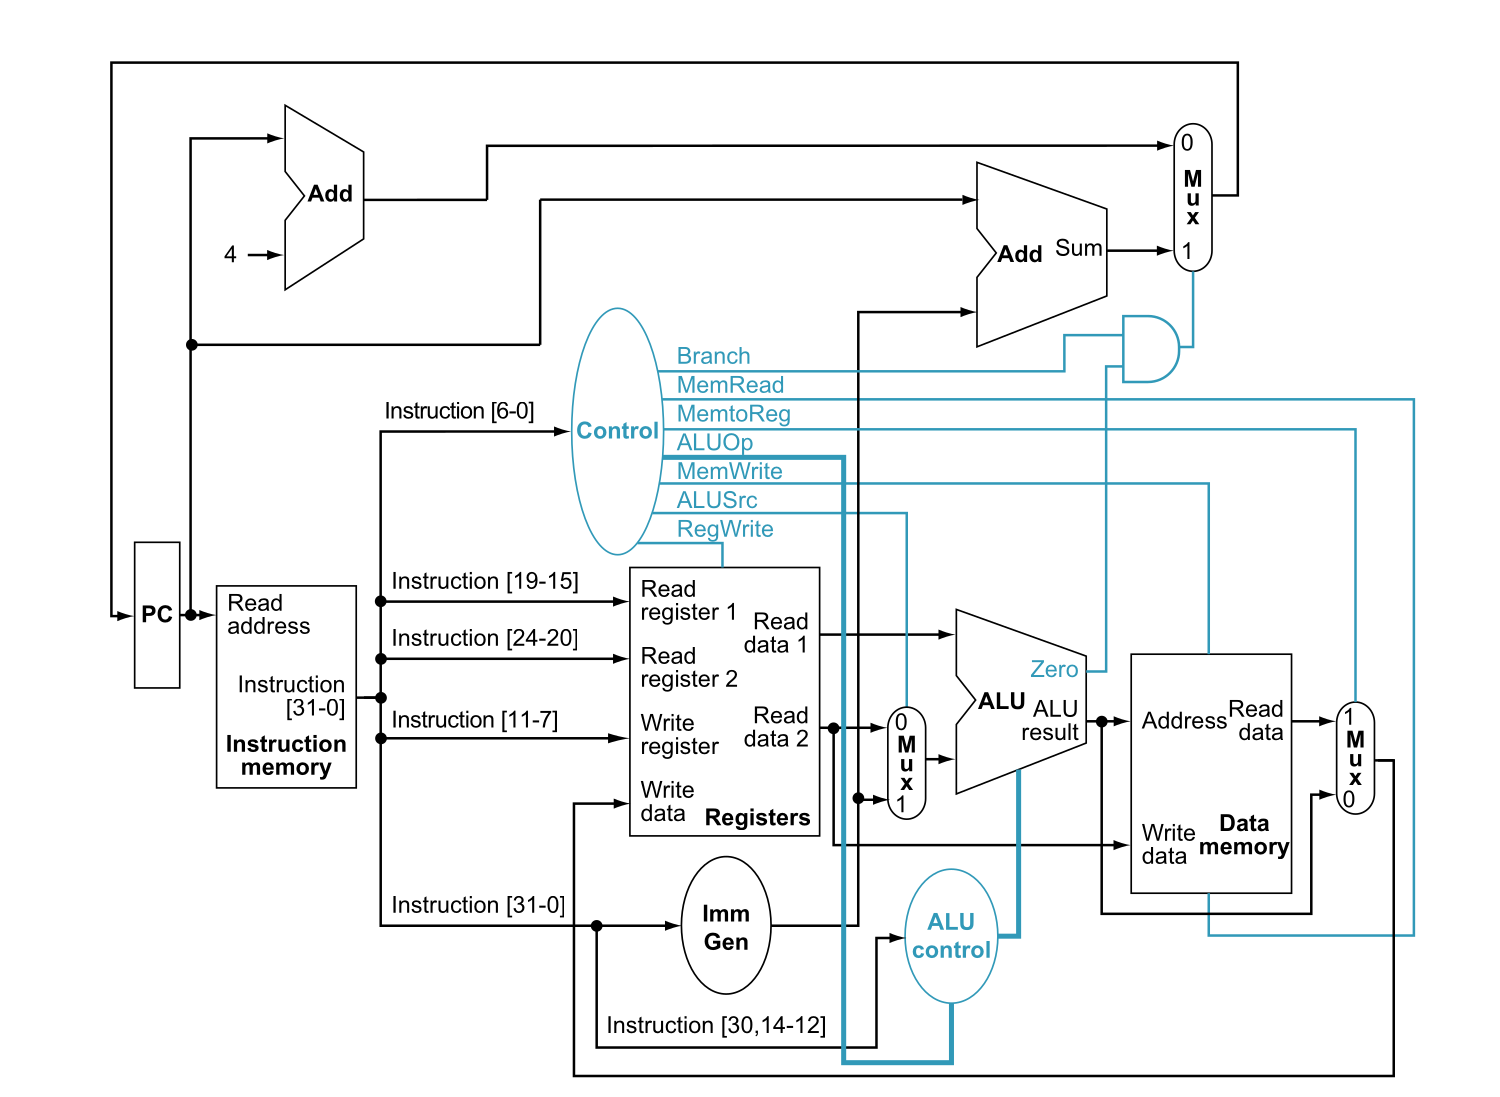
\includegraphics[width=\textwidth]{hannersy-patterson-implementation-fig4-21.png}
\fonte[Source]{Figure 4.21 of \citeonline{patterson2020} --- David A. Patterson
  and John L. Hennessy, \emph{Computer Organization and Design: RISC-V
  Edition}, 2nd ed., Morgan Kaufmann (an imprint of Elsevier), 2020.
  Reproduced here for academic purposes; copyright in the original
  illustration remains with the authors and the publisher.}
\nota[Note]{Black lines carry values and blue lines carry control signals.
  The subset has no upper-immediate path into the register file
  (\texttt{lui}), no \mbox{PC~+~4} write-back into the register file
  (\texttt{jal}, \texttt{jalr}), no register~$\rightarrow$~PC path
  (\texttt{jalr}) and no path from the \mbox{PC~+~immediate} adder into the
  register file, which only steers the PC multiplexer (\texttt{auipc}); each
  of those absences is the hardware reason for a synthesis derived in
  Section~\ref{sec:sc1-synthesis}.}
\end{figure}


The two absences that matter most for a compiler are visible in the figure as multiplexer inputs that
were never built. Without an upper-immediate input to the write-back multiplexer there is no single
instruction that places a large constant in a register, and without a PC-to-register path there is no
instruction that records a return address, which is what makes function calls impossible on rvsc0
(Section~\ref{sec:sc0-no-calls}). Every other restriction the subset imposes is an absent decode case
rather than an absent wire: the ALU and the branch comparator are already there, so \texttt{xor}, the
shifts and the ordered branches can be rebuilt out of the operations the datapath does route.

\section{C Calling Convention and ABI}

An Application Binary Interface (ABI) is the binary-level contract that allows separately compiled
translation units to interoperate. It specifies which registers hold function arguments, which the
caller must preserve across a call, which the callee must preserve, how the stack is laid out, and how
values are returned. Code compiled by different compilers for the same ABI can be linked and executed
together.

The RISC-V integer ABI partitions the 32 registers into four groups \cite{riscv-psabi}. Argument and
return-value registers (a0--a7, i.e.\ x10--x17) pass the first eight integer arguments to a function
and carry the return value back in a0 (and a1 for 64-bit values on RV32). Caller-saved temporaries
(t0--t6, i.e.\ x5--x7 and x28--x31) may be freely overwritten by any callee; the caller must save
them if their values are needed after a call. Callee-saved registers (s0--s11, i.e.\ x8--x9 and
x18--x27) must be preserved across calls; a callee that uses them must save and restore them.
Special-purpose registers are: ra (x1) the return address, sp (x2) the stack pointer, gp (x3) the
global pointer, and tp (x4) the thread pointer.

\begin{table}[htb]
\centering
\caption{RISC-V integer register conventions \cite{riscv-psabi}}
\label{tab:riscv-registers}
\begin{tabular}{llll}
\toprule
\textbf{Register} & \textbf{ABI name} & \textbf{Role} & \textbf{Saved by} \\
\midrule
x0        & zero    & Hardwired zero       & --- \\
x1        & ra      & Return address       & Caller \\
x2        & sp      & Stack pointer        & Callee \\
x3        & gp      & Global pointer       & --- \\
x4        & tp      & Thread pointer       & --- \\
x5--x7    & t0--t2  & Temporaries          & Caller \\
x8--x9    & s0--s1  & Saved registers      & Callee \\
x10--x11  & a0--a1  & Args / return value  & Caller \\
x12--x17  & a2--a7  & Arguments            & Caller \\
x18--x27  & s2--s11 & Saved registers      & Callee \\
x28--x31  & t3--t6  & Temporaries          & Caller \\
\bottomrule
\end{tabular}
\end{table}

The RISC-V stack grows downward. A typical stack frame contains, from high to low address: incoming
arguments that did not fit in a0--a7, the saved return address, saved callee-saved registers, and local
variables. The call sequence is: the caller loads arguments into a0--a7 (and pushes any extras onto
the stack), then executes \texttt{jal ra, target} to jump to the callee and record the return address
in ra. The callee saves ra and any s registers it uses, executes its body, places the result in a0,
restores saved registers, and returns with \texttt{jalr x0, 0(ra)} (the \texttt{ret}
pseudo-instruction). The stack pointer must be 16-byte aligned at every function entry and exit
\cite{riscv-psabi}.

GCC emits ELF (Executable and Linkable Format) object files. The principal sections are \texttt{.text}
(machine code), \texttt{.rodata} (read-only constants and string literals), \texttt{.data} (initialized
global variables), and \texttt{.bss} (zero-initialized global variables). Relocation entries in the
object file record every reference to a symbol whose address is not yet known; the linker fills these
in when it combines object files. A linker script controls the memory layout: it assigns each section
to an address range that matches the target processor's address map \cite{riscv-psabi}.

\section{GCC Compiler Architecture}

The GNU Compiler Collection (GCC) is a portable, multi-language, multi-target compiler and the
dominant toolchain for embedded and systems software \cite{gcc-internals}. It translates C (and other
languages) to machine code through a sequence of intermediate representations that progressively lower
the abstraction level.

The compilation pipeline proceeds as follows \cite{gcc-internals}, and is summarised in
Figure~\ref{fig:pipeline}. The language frontend parses source
code and produces an abstract syntax tree (AST). The AST is lowered to GIMPLE, a high-level,
language-independent, statement-level intermediate representation in static single-assignment (SSA)
form. The middle-end applies target-independent optimisations to GIMPLE (constant folding, inlining,
loop transformations, and others). GIMPLE is then lowered to RTL (Register Transfer Language), a
low-level IR that models instructions as operations on pseudo-registers and memory. The backend
operates on RTL to produce assembly.

The backend performs three main tasks \cite{gcc-internals}. Instruction selection pattern-matches RTL
expressions against the target's machine description to select real instructions. Register allocation
assigns the potentially unbounded set of pseudo-registers to the finite set of physical registers,
inserting spill code where necessary. Instruction scheduling reorders instructions to hide pipeline
latency and improve throughput; it is irrelevant for single-cycle processors, which have no pipeline
and therefore no data hazards.

The core of a GCC backend is the machine description file (\texttt{.md}), which declaratively
specifies the target's instruction set and expansion rules \cite{gcc-internals}. It contains two
primary construct types:

\begin{itemize}
  \item \texttt{define\_insn}: specifies a named RTL pattern, an assembly output template, and a
        predicate condition string that tests target capabilities. When the condition evaluates to
        false, the pattern is invisible to the instruction selector and will never be emitted.
  \item \texttt{define\_expand}: specifies a named operation that expands into an arbitrary sequence
        of RTL insns when the compiler needs to generate that operation. The expansion body may call
        \texttt{DONE} to signal that it has produced the complete implementation, preventing any
        fallthrough to a \texttt{define\_insn}. Expansions are the mechanism used to synthesize
        complex operations from simpler ones.
\end{itemize}

Code iterators (such as \texttt{any\_shift}) allow a single \texttt{define\_expand} to cover multiple
related operations (ASHIFT, LSHIFTRT, ASHIFTRT) in one body, with runtime-constant guards like
\texttt{(<CODE>) == ASHIFT} selecting the appropriate synthesis path.

% GCC compilation pipeline, marking the point where this work's synthesis
% happens (the RTL expansion pass, where `define_expand` bodies run).
%
% TikZ port of figures/pipeline.typ.  Conventions:
%   - solid boxes / arrows : the representations and the passes between them
%   - dashed grey boxes    : machine-description constructs acting at that step
\begin{figure}[htb]
\centering
\begin{SingleSpace}
\begin{tikzpicture}[
  x=0.74cm, y=0.74cm,
  font=\sffamily\fontsize{7}{8}\selectfont,
  stage/.style={draw, fill=black!4, inner sep=0pt, align=center,
                line width=0.5pt},
  flow/.style={-{Straight Barb[scale=0.55]}, line width=0.5pt},
  note/.style={draw=black!45, dashed, line width=0.4pt},
  notetext/.style={anchor=north west, text=black!55, align=left,
                   font=\sffamily\fontsize{5.5}{6.6}\selectfont},
  passlbl/.style={anchor=east, align=right,
                  font=\sffamily\fontsize{5.5}{6.6}\selectfont},
  bracket/.style={draw=black!50, line width=0.5pt},
]

\def\bxa{2.2}
\def\bxb{6.4}
\def\ax{4.3}

\newcommand{\Stage}[2]{%
  \path[stage] (\bxa,{#1-0.45}) rectangle (\bxb,{#1+0.45});
  \node at ({(\bxa+\bxb)/2},#1) {#2};}
% Vertical arrow between two stages, with the pass name to its left.
\newcommand{\Step}[3]{%
  \draw[flow] (\ax,{#1-0.45}) -- (\ax,{#2+0.45});
  \node[passlbl] at ({\ax-0.25},{(#1+#2)/2}) {#3};}
% Dashed note box on the right, with a pointer into the flow.
\newcommand{\Note}[4]{%
  \path[note] (10.2,#1) rectangle (18.1,#2);
  \node[notetext] at (10.4,{#1-0.2}) {#4};
  \draw[note, -{Straight Barb[scale=0.5]}] (10.2,#3) -- ({\ax+0.15},#3);}
% Phase bracket down the left-hand side.
\newcommand{\Phase}[3]{%
  \draw[bracket] (-0.5,#1) -- (-0.5,#2);
  \draw[bracket] (-0.5,#1) -- (-0.3,#1);
  \draw[bracket] (-0.5,#2) -- (-0.3,#2);
  \node[rotate=-90, text=black!60,
        font=\sffamily\fontsize{5.5}{6.6}\selectfont]
    at (-0.85,{(#1+#2)/2}) {#3};}

% --- the representations -------------------------------------------------
\Stage{0}{C source}
\Stage{-1.9}{GENERIC (AST)}
\Stage{-3.9}{GIMPLE, SSA form}
\Stage{-6.3}{RTL, pseudo-registers}
\Stage{-8.4}{RTL, hard registers}
\Stage{-10.2}{assembly (\texttt{.s})}
\Stage{-12.0}{ELF object}

% --- the passes between them ---------------------------------------------
\Step{0}{-1.9}{parse}
\Step{-1.9}{-3.9}{gimplify,\\SSA construction}
\Step{-3.9}{-6.3}{\textbf{RTL expansion}}
\Step{-6.3}{-8.4}{combine, register\\allocation (IRA/LRA),\\post-reload splits}
\Step{-8.4}{-10.2}{final: output\\templates}
\Step{-10.2}{-12.0}{\texttt{as} (binutils)}

\node[anchor=west, text=black!60, align=left,
      font=\sffamily\fontsize{5.5}{6.6}\selectfont\itshape]
  at ({\bxb+0.3},-3.9) {target-independent\\optimisation passes};

% --- phase brackets -------------------------------------------------------
\Phase{0.5}{-4.4}{front end + middle end}
\Phase{-4.9}{-10.7}{back end (target dependent)}

% --- what the machine description contributes, and where ------------------
\path[note] (10.2,0.5) rectangle (18.1,-1.15);
\node[notetext] at (10.4,0.3) {%
  \texttt{rvscN.h} \texttt{CC1\_SPEC} injects \texttt{-mno-shift},
  \texttt{-mno-xor}, \dots\\
  which clear the \texttt{riscv.opt} flags \texttt{TARGET\_SHIFT},\\
  \texttt{TARGET\_XOR}, \dots\ tested by every condition below};
\draw[note, -{Straight Barb[scale=0.5]}] (13.4,-1.15) -- (13.4,-3.7);

\Note{-3.7}{-5.7}{-5.1}{%
  \texttt{define\_expand} --- \textbf{where the synthesis happens.}\\
  With \texttt{-mno-shift}, \texttt{ashlsi3} expands to a chain of
  \texttt{add}\\
  instructions and calls \texttt{DONE}, so the \texttt{sll} pattern is never\\
  reached: the operation ceases to exist as RTL.}
\Note{-6.5}{-8.0}{-7.35}{%
  \texttt{define\_insn\_and\_split} --- splits that must run\\
  after register allocation, such as replacing\\
  \texttt{andi rd,rs,0xff} by \texttt{li} + \texttt{and}.}
\Note{-8.5}{-10.0}{-9.3}{%
  \texttt{define\_insn} --- output templates. A pattern whose\\
  condition is false (\texttt{TARGET\_SHIFT} on rvsc1) is\\
  invisible to instruction selection.}

\end{tikzpicture}

\vspace{0.4em}
{\footnotesize\color{black!60}\raggedright
The RTL expansion pass is where the synthesis of this work happens: a
\texttt{define\_expand} guarded by a \texttt{-mno-} flag emits a replacement
sequence and calls \texttt{DONE}, so the absent instruction never enters RTL and
no later pass can reintroduce it.\par}

\end{SingleSpace}
\caption{GCC compilation pipeline and the machine-description construct acting
         at each step}
\label{fig:pipeline}
\end{figure}


The position of that expansion step in the pipeline determines what the rest of this work can and
cannot do. Because synthesis happens as GIMPLE is lowered to RTL, every subsequent pass, register
allocation included, sees only the replacement sequence and optimises it as ordinary code, which is
what makes the synthesis transparent. The same position also explains the loss discussed in
Section~\ref{sec:sc1-corner-cases}: once an \texttt{xor} has become an \texttt{and}, an \texttt{or} and
a \texttt{sub}, no later pass can recognise the algebraic identities of the operation it replaced, so
any identity worth exploiting must be folded inside the expansion body itself.

Target-specific command-line options are declared in a \texttt{.opt} file using GCC's
option-description syntax \cite{gcc-internals}. Each declaration generates a C preprocessor macro
that can be tested in \texttt{.md} condition strings and in C target-hook implementations. A
per-target header file defines \texttt{CC1\_SPEC}, a GCC macro evaluated when the driver invokes the
compiler proper (\texttt{cc1}). It contains conditional option-injection rules of the form ``if the
user did not explicitly pass a flag, inject its negation.'' This mechanism makes a target
self-configuring: users invoke the target-specific compiler without any manual flags, and the correct
behaviour is activated automatically.


% Chapter 3. Development Method
\chapter{Development Method} \label{cap:method}

This work followed an iterative process organized into four phases: a study phase to understand GCC's
backend architecture, a requirements phase to define the instruction boundaries for each target, a
per-synthesis implementation-and-test cycle that forms the core of the work, and a validation phase
that confirms behavioral correctness on a reference simulator. Chapter~\ref{cap:requirements},
Chapter~\ref{cap:development}, and Chapter~\ref{cap:results} describe the outputs of these phases in
detail; this chapter describes the process itself.

\section{Study of GCC Internals}

The first phase was a structured study of GCC's backend extension mechanisms. The entry point was the
GCC Internals manual \cite{gcc-internals}, which documents the machine description language
(\texttt{.md}), the option description system (\texttt{.opt}), and the role of per-target
configuration headers. After establishing a conceptual model from the manual, the existing RISC-V
backend (\texttt{gcc/config/riscv/riscv.md}, \texttt{riscv.opt}, and \texttt{config.gcc}) was
examined as a working reference implementation.

Two diagnostic tools were central throughout the study and subsequent implementation phases. The
\texttt{-S} flag causes GCC to emit assembly rather than an object file, making the compiler's
instruction selection directly observable. The \texttt{-fdump-rtl-*} family of flags produces
snapshots of GCC's internal Register Transfer Language (RTL) representation at each compilation
stage; these were used to understand why a pattern matched or failed to match during instruction
selection, and to verify that \texttt{define\_expand} bodies fired at the correct point in the
compilation pipeline.

\section{Requirements Specification}

Requirements for each target were derived from two sources. For rvsc0 and rvsc1, the instruction
boundaries are externally fixed by the Hennessy-Patterson textbook \cite{patterson2020} and the
minimum ABI requirements, respectively. For rvsc2--rvsc7, the boundaries follow the natural RISC-V
extension hierarchy \cite{riscv-spec}. The complete requirements are specified in
Chapter~\ref{cap:requirements}.

\section{Synthesis Derivation and Implementation}

The rvsc0 and rvsc1 targets require GCC to synthesize every instruction outside the native set using
only the instructions the processor supports. Each synthesis was developed through the following cycle,
applied independently to each missing operation.

The process begins by identifying the missing operation, an instruction that GCC's middle-end may
legally request but that the target processor does not support. The synthesis algorithm is then derived
and expressed as C pseudocode, which serves both as a correctness argument and as an unambiguous
specification of the target behavior. The pseudocode is then lifted directly into a
\texttt{define\_expand} body in \texttt{riscv.md}, using GCC's RTL emit helpers to generate the
equivalent sequence of native instructions. Correctness of the expansion is confirmed in two steps:
the \texttt{-S} output is inspected to verify that no forbidden mnemonics appear, and the resulting
program is executed on the Spike RISC-V ISA simulator \cite{spike} to confirm that the synthesized
sequence produces the same result as the original instruction would have.

This cycle was repeated for each operation that the compiler may emit for a bare-metal freestanding C
program targeting rvsc0 or rvsc1. The derivations and the resulting implementation are described in
Chapter~\ref{cap:development}.

\section{Validation}

Validation addresses two correctness requirements defined in Chapter~\ref{cap:requirements}: ISA
compliance and behavioral equivalence.

ISA compliance is verified structurally by disassembling the compiled output and checking every
mnemonic against a per-target allowlist.

Behavioral equivalence is verified by differential execution: the same C program is compiled by both
the custom target and a reference RV32I compiler, and both binaries are executed on the Spike ISA
simulator \cite{spike}; the test passes when both produce identical exit codes.

A third validation layer exercises the compiler against a much larger, automatically generated corpus.
The GCC test suite includes a \textit{torture test} mode that systematically varies optimization flags
and source patterns across hundreds of programs; besides compiling \texttt{libgcc} against the custom
target also stresses constant materialization, multi-word arithmetic, and calling-convention edge cases
that hand-written behavioral tests would not cover.

Test results are presented in Chapter~\ref{cap:results}.


% Chapter 4. Requirements Specification
\chapter{Requirements Specification} \label{cap:requirements}

This chapter defines the requirements for the eight GCC cross-compiler targets developed in this work.
Each target is a modified GCC backend that accepts bare-metal freestanding C programs and produces
machine code containing only the instructions supported by the corresponding educational processor.

\section{Scope}

All targets compile \textbf{bare-metal freestanding C}: programs with no standard library and no
operating system, producing an ELF binary as output.

\section{Correctness Requirements}

Two independent correctness requirements apply to every target.

\textbf{ISA compliance}: the compiler must never emit an instruction whose opcode is not in the
target's allowed set. This requirement is verifiable by inspecting the assembly output.

\textbf{Behavioral equivalence}: the compiled program must exhibit the same observable behavior as
the source --- the same return values, the same memory effects, and the same control flow --- as if
compiled for a processor that natively supports the full instruction set.

\section{rvsc0 --- Basic Single-Cycle}

The rvsc0 target corresponds to the eight-instruction single-cycle processor described in Chapter 4.4
of \cite{patterson2020}, \textit{A Simple Implementation Scheme}:

\begin{quote}
In this section, we look at what might be thought of as a simple implementation of our RISC-V subset.
[\ldots] This simple implementation covers load word (lw), store word (sw), branch if equal (beq),
and the arithmetic-logical instructions add, sub, and, and or.
\end{quote}

\begin{table}[htb]
\centering
\caption{rvsc0 native instruction set}
\label{tab:rvsc0-isa}
\begin{tabular}{ll}
\toprule
\textbf{Mnemonic} & \textbf{Description} \\
\midrule
\texttt{lw}   & Load word \\
\texttt{sw}   & Store word \\
\texttt{beq}  & Branch if equal \\
\texttt{add}  & Add \\
\texttt{addi} & Add immediate \\
\texttt{sub}  & Subtract \\
\texttt{and}  & Bitwise AND \\
\texttt{or}   & Bitwise OR \\
\bottomrule
\end{tabular}
\end{table}

\subsection{Limitations}

The rvsc0 processor has no mechanism to write the program counter --- it supports neither \texttt{jalr}
nor any jump-and-link instruction. As a consequence, subroutine calls are architecturally impossible,
and the set of C programs that can be compiled for rvsc0 is restricted accordingly. For all other C
constructs, the compiler must produce correct behavior using only the native instruction set.

\section{rvsc1 --- Extended Single-Cycle}

The rvsc1 target extends rvsc0 with \texttt{lui} and \texttt{jalr}. These two instructions are the
minimum addition that enables the full C calling convention: \texttt{lui} materializes 32-bit absolute
addresses and \texttt{jalr} performs indirect jumps and encodes function returns via
\texttt{jalr x0, 0(ra)}.

\begin{table}[htb]
\centering
\caption{rvsc1 native instruction set}
\label{tab:rvsc1-isa}
\begin{tabular}{ll}
\toprule
\textbf{Mnemonic} & \textbf{Description} \\
\midrule
\texttt{lw}   & Load word \\
\texttt{sw}   & Store word \\
\texttt{beq}  & Branch if equal \\
\texttt{add}  & Add \\
\texttt{addi} & Add immediate \\
\texttt{sub}  & Subtract \\
\texttt{and}  & Bitwise AND \\
\texttt{or}   & Bitwise OR \\
\texttt{lui}  & Load upper immediate \\
\texttt{jalr} & Jump and link register \\
\bottomrule
\end{tabular}
\end{table}

With these ten instructions, the target must support the full C calling convention and general-purpose
C programs.

\section{rvsc2 --- Single-Cycle Without Fence and Control}

The rvsc2 target implements the full RV32I base ISA with three groups of instructions excluded. Memory
ordering instructions are unnecessary on a single-core single-cycle processor: omitting them is
behavior-preserving. CSR access and system instructions require operating system support that is absent
in the bare-metal environment.

\begin{table}[htb]
\centering
\caption{rvsc2 native instruction set (RV32I base, excluding fence, CSR, and system groups)}
\label{tab:rvsc2-isa}
\begin{tabular}{ll}
\toprule
\textbf{Group} & \textbf{Instructions} \\
\midrule
Integer arithmetic & \texttt{add, sub, addi, and, andi, or, ori, xor, xori, sll, slli, srl, srli, sra, srai} \\
Comparison         & \texttt{slt, sltu, slti, sltiu} \\
Loads              & \texttt{lw, lh, lhu, lb, lbu} \\
Stores             & \texttt{sw, sh, sb} \\
Branches           & \texttt{beq, bne, blt, bge, bltu, bgeu} \\
Jumps              & \texttt{jal, jalr} \\
Upper immediate    & \texttt{lui, auipc} \\
\bottomrule
\end{tabular}
\end{table}

\begin{table}[htb]
\centering
\caption{rvsc2 instruction treatment}
\label{tab:rvsc2-treatment}
\begin{tabular}{ll}
\toprule
\textbf{Treatment} & \textbf{Instructions} \\
\midrule
Behaviorally equivalent & \texttt{fence, fence.i, sfence.vma} \\
Rejected & \texttt{ecall, ebreak, sret, wfi}, CSR instructions (\texttt{csrrw, csrrs, csrrc, csrrwi, csrrsi, csrrci}) \\
\bottomrule
\end{tabular}
\end{table}

\section{rvsc3 --- Single-Cycle rv32i}

The rvsc3 target implements the complete RV32I base integer ISA \cite{riscv-spec}, including the
memory ordering, CSR access, and system instruction groups omitted from rvsc2. No instruction
synthesis is required: every RV32I instruction is natively supported by the hardware.

\begin{table}[htb]
\centering
\caption{rvsc3 native instruction set (complete RV32I)}
\label{tab:rvsc3-isa}
\begin{tabular}{ll}
\toprule
\textbf{Group} & \textbf{Instructions} \\
\midrule
Integer arithmetic & \texttt{add, sub, addi, and, andi, or, ori, xor, xori, sll, slli, srl, srli, sra, srai} \\
Comparison         & \texttt{slt, sltu, slti, sltiu} \\
Loads              & \texttt{lw, lh, lhu, lb, lbu} \\
Stores             & \texttt{sw, sh, sb} \\
Branches           & \texttt{beq, bne, blt, bge, bltu, bgeu} \\
Jumps              & \texttt{jal, jalr} \\
Upper immediate    & \texttt{lui, auipc} \\
Memory ordering    & \texttt{fence, fence.i} \\
System             & \texttt{ecall, ebreak, wfi, sret} \\
CSR                & \texttt{csrrw, csrrs, csrrc, csrrwi, csrrsi, csrrci} \\
\bottomrule
\end{tabular}
\end{table}

\section{rvsc4 --- Single-Cycle rv64i}

The rvsc4 target is a 64-bit processor implementing the full rv64i instruction set. In addition to all
rvsc3 instructions, it natively supports:

\begin{itemize}
  \item 64-bit memory operations: \texttt{ld}, \texttt{sd}, \texttt{lwu}
  \item Word operations with sign-extended 64-bit results: \texttt{addw}, \texttt{subw},
        \texttt{addiw}, \texttt{sllw}, \texttt{srlw}, \texttt{sraw}, \texttt{slliw},
        \texttt{srliw}, \texttt{sraiw}
\end{itemize}

The W-suffix variants operate on 32 bits and sign-extend the result to 64 bits, following the same
convention as \texttt{addw}, \texttt{subw}, and the other W instructions from rvsc4.

\section{rvsc5 --- Single-Cycle rv64im}

The rvsc5 target extends rvsc4 with the M extension, adding native integer multiply and divide:

\begin{itemize}
  \item Multiply: \texttt{mul, mulw, mulh, mulhu, mulhsu}
  \item Signed divide: \texttt{div, divw}
  \item Unsigned divide: \texttt{divu, divuw}
  \item Signed remainder: \texttt{rem, remw}
  \item Unsigned remainder: \texttt{remu, remuw}
\end{itemize}

\section{rvsc6 --- Single-Cycle Floating-Point}

The rvsc6 target extends rvsc5 with the complete F (single-precision) and D (double-precision)
floating-point extensions as defined in \cite{riscv-spec}, supporting all arithmetic, memory,
conversion, and comparison instructions for both precisions.

\begin{itemize}
  \item Loads/stores: \texttt{flw, fsw} (single); \texttt{fld, fsd} (double)
  \item Arithmetic: \texttt{fadd.s, fadd.d, fsub.s, fsub.d, fmul.s, fmul.d, fdiv.s, fdiv.d,
        fsqrt.s, fsqrt.d}
  \item Fused multiply-add: \texttt{fmadd.s, fmadd.d, fmsub.s, fmsub.d, fnmadd.s, fnmadd.d,
        fnmsub.s, fnmsub.d}
  \item Sign, minimum, maximum: \texttt{fsgnj.s, fsgnj.d, fsgnjn.s, fsgnjn.d, fsgnjx.s, fsgnjx.d,
        fmin.s, fmin.d, fmax.s, fmax.d}
  \item Comparison and classification: \texttt{feq.s, feq.d, flt.s, flt.d, fle.s, fle.d,
        fclass.s, fclass.d}
  \item Move between integer and FP registers: \texttt{fmv.w.x, fmv.x.w} (single);
        \texttt{fmv.d.x, fmv.x.d} (double)
  \item Conversions (rv64): \texttt{fcvt.s.w, fcvt.s.wu, fcvt.s.l, fcvt.s.lu} (int to single);
        \texttt{fcvt.w.s, fcvt.wu.s, fcvt.l.s, fcvt.lu.s} (single to int);
        \texttt{fcvt.d.w, fcvt.d.wu, fcvt.d.l, fcvt.d.lu} (int to double);
        \texttt{fcvt.w.d, fcvt.wu.d, fcvt.l.d, fcvt.lu.d} (double to int);
        \texttt{fcvt.s.d, fcvt.d.s} (between single and double)
\end{itemize}

\section{rvsc7 --- Single-Cycle Atomic}

The rvsc7 target extends rvsc6 with the A extension (atomic memory operations), implementing the full
rv64imafd instruction set \cite{riscv-spec}. The \texttt{.w} variants operate on 32 bits
(sign-extended to 64); the \texttt{.d} variants operate on 64 bits.

\begin{itemize}
  \item Load-reserved and store-conditional: \texttt{lr.w, lr.d}; \texttt{sc.w, sc.d}
  \item AMO (atomic memory operations):
        \texttt{amoadd.w, amoadd.d} (atomic add);
        \texttt{amoand.w, amoand.d} (atomic AND);
        \texttt{amoor.w, amoor.d} (atomic OR);
        \texttt{amoxor.w, amoxor.d} (atomic XOR);
        \texttt{amoswap.w, amoswap.d} (atomic swap);
        \texttt{amomax.w, amomax.d} (atomic signed maximum);
        \texttt{amomaxu.w, amomaxu.d} (atomic unsigned maximum);
        \texttt{amomin.w, amomin.d} (atomic signed minimum);
        \texttt{amominu.w, amominu.d} (atomic unsigned minimum)
\end{itemize}


% Chapter 5. Development
\chapter{Development} \label{cap:development}

The rvsc0 and rvsc1 targets restrict the instruction set available to the compiler
(Chapter~\ref{cap:requirements} specifies the complete native instruction set for each target). Every
C construct the compiler may emit must be realized using only those native instructions; for every
excluded instruction, GCC synthesizes an equivalent sequence at compile time. This chapter presents
the tools and infrastructure used, the mathematical derivation and proof of each synthesis, the GCC
implementation that makes the process transparent to the programmer, and the known limitations of each
target.

\section{Technologies Used}

\subsection{GCC 17.0.0}

The custom targets are implemented as a backend extension to GCC 17.0.0. GCC is chosen because it is
the dominant open-source compiler for embedded and systems software and because its machine description
framework provides a declarative mechanism for defining instruction synthesis rules that is already
present in the upstream RISC-V backend. The following files in the GCC source tree were modified or
added:

\begin{table}[htb]
\centering
\caption{GCC source files modified or added for this project}
\label{tab:gcc-files}
\begin{tabular}{ll}
\toprule
\textbf{File} & \textbf{Role} \\
\midrule
\texttt{gcc/config/riscv/riscv.md}  & Machine description: synthesis patterns and native instruction guards \\
\texttt{gcc/config/riscv/riscv.opt} & Option declarations: per-synthesis boolean flags \\
\texttt{gcc/config/riscv/riscv.cc}  & Target hooks: addi/shift constant synthesis for LUI \\
\texttt{gcc/config/riscv/rvscN.h}   & Per-target headers: \texttt{CC1\_SPEC} injecting \texttt{-mno-*} flags automatically \\
\texttt{gcc/config/config.gcc}      & Triple mapping: \texttt{rvscN-*-elf*} to \texttt{cpu\_type=riscv} \\
\texttt{gcc/config/config.sub}      & Triple normalisation: recognises \texttt{rvscN} as a valid CPU name \\
\bottomrule
\end{tabular}
\end{table}

\subsection{GNU Binutils (riscv32/64-none-elf)}

The upstream GNU binutils cross toolchain is used without modification as the assembler and linker.
The binutils triple differs from the compiler triple: \texttt{riscv32-none-elf} for rvsc0--rvsc3 and
\texttt{riscv64-none-elf} for rvsc4--rvsc7.

\subsection{Spike 1.1.1-dev}

Spike is the official RISC-V ISA reference simulator \cite{spike}. It implements the full
RV64IMAFD instruction set, making it suitable as the behavioral oracle: a binary compiled by
\texttt{rvsc1-unknown-elf-gcc} contains only valid RV32I instructions (the synthesis sequences are
themselves valid RV32I), so Spike can execute it and report the correct result. Spike is invoked with
\texttt{--isa=rv32i} for rvsc0--rvsc3 tests, and with \texttt{--log-commits} to count retired
instructions for performance measurements.

\section{Toolchain Installation}

\subsection{Repository Setup}

The GCC backend modifications live in a fork of the upstream GCC repository:

\begin{lstlisting}[language=bash]
git clone https://github.com/guissalustiano/gcc-hannersy-paterson gcc
\end{lstlisting}

The GNU Binutils source is cloned separately and is required for all targets, since GCC must invoke
the target assembler during compilation:

\begin{lstlisting}[language=bash]
git clone https://sourceware.org/git/binutils-gdb.git binutils-gdb
\end{lstlisting}

Both repositories should sit side by side in the same parent directory. The build directories and
installed toolchains are placed inside a per-target subdirectory:

\begin{lstlisting}
project/
+-- gcc/              <- GCC fork (source, never built in-tree)
+-- binutils-gdb/     <- binutils source
+-- targets/
    +-- rvsc2/
        +-- build-binutils/   <- binutils out-of-tree build
        +-- build/            <- GCC out-of-tree build
        +-- install/          <- installed toolchain (bin/, lib/, ...)
\end{lstlisting}

\subsection{Building Binutils}

Binutils must be built and installed before GCC so that GCC's configure step can detect the target
assembler and linker.

\begin{lstlisting}[language=bash]
mkdir -p targets/rvsc2/build-binutils
cd targets/rvsc2/build-binutils

../../binutils-gdb/configure \
    --target=rvsc2-unknown-elf \
    --prefix=$(pwd)/../install \
    --disable-nls \
    --disable-gdb

make -j$(nproc)
make install
\end{lstlisting}

After this step the install prefix contains the target assembler, linker, and binutils utilities
(\texttt{rvsc2-unknown-elf-as}, \texttt{rvsc2-unknown-elf-ld}, etc.).

\subsection{Building GCC}

With the assembler and linker installed, GCC can be configured and built. The three
\texttt{--disable-*} flags prevent GCC from attempting to rebuild its own copies of the binutils
components from the source tree (the GCC repository bundles a copy of binutils), which avoids
duplicate build failures and unnecessary compilation time.

\begin{lstlisting}[language=bash]
mkdir -p targets/rvsc2/build
cd targets/rvsc2/build

PATH="$(pwd)/../install/bin:$PATH" \
../../gcc/configure \
    --target=rvsc2-unknown-elf \
    --prefix=$(pwd)/../install \
    --enable-languages=c \
    --with-newlib \
    --disable-binutils \
    --disable-ld \
    --disable-gas

make all-gcc -j$(nproc)
make install-gcc
\end{lstlisting}

Prepending the install prefix to \texttt{PATH} before configure allows the configure script to detect
the pre-installed \texttt{rvsc2-unknown-elf-as} and \texttt{rvsc2-unknown-elf-ld} binaries, preventing
it from scheduling them for in-tree compilation.

\subsection{Building Newlib and libgcc}

With GCC installed, the C runtime library (newlib) and the compiler support library (libgcc) can be
built. Both are required to link executable programs.

\begin{lstlisting}[language=bash]
mkdir -p targets/rvsc2/build-newlib
cd targets/rvsc2/build-newlib

PATH="$(pwd)/../install/bin:$PATH" \
../../newlib-src/configure \
    --target=rvsc2-unknown-elf \
    --prefix=$(pwd)/../install \
    --disable-multilib \
    --disable-newlib-supplied-syscalls

PATH="$(pwd)/../install/bin:$PATH" make -j$(nproc)
PATH="$(pwd)/../install/bin:$PATH" make install
\end{lstlisting}

With newlib installed, libgcc can be built against it:

\begin{lstlisting}[language=bash]
cd targets/rvsc2/build

PATH="$(pwd)/../install/bin:$PATH" make all-target-libgcc -j$(nproc)
PATH="$(pwd)/../install/bin:$PATH" make install-target-libgcc
\end{lstlisting}

After all four steps the toolchain is fully self-contained under \texttt{targets/rvsc2/install/bin/}.
Compiling a C program to a RISC-V object file requires only:

\begin{lstlisting}[language=bash]
PATH="targets/rvsc2/install/bin:$PATH" \
rvsc2-unknown-elf-gcc -O2 -ffreestanding -c program.c -o program.o
\end{lstlisting}

\section{Synthesis Derivations} \label{sec:sc1-synthesis}

\textbf{Assembly notation.} In the listings below, \texttt{rd}, \texttt{rs1}, and \texttt{rs2} denote
the canonical destination and source registers. Registers \texttt{t0}--\texttt{t5} are temporaries
chosen for readability. In the actual GCC machine description, all temporaries are allocated as
pseudo-registers via \texttt{gen\_reg\_rtx(SImode)}. The register allocator maps them to physical
registers, resolving aliasing conflicts automatically. The bracket notation \texttt{[op ...]} marks
an instruction that is itself synthesized, its expansion is defined in the subsection that covers that
operation.

\subsection{Arithmetic}

Arithmetic synthesis operations assign values only to registers and carry no memory side-effects. They
can be replaced by equivalent sequences without additional constraints.

\subsubsection{Bitwise NOT} \label{sec:sc1-not}

The standard RISC-V pseudo-instruction \texttt{not rd, rs1} expands to \texttt{xori rd, rs1, -1}.
Neither sc0 nor sc1 include \texttt{xori}, so a different derivation is required.

\textbf{Proof.} In two's complement, negation satisfies $-x = \mathord{\sim}x + 1$ for all $x$.
Rearranging: $\mathord{\sim}x = -x - 1$. Both subtraction from zero (\texttt{sub rd, x0, rs1}) and
decrement by one (\texttt{addi rd, rd, -1}) are available in sc0 and sc1. $\square$

\begin{lstlisting}
sub  rd, x0, rs1    # rd = -rs1
addi rd, rd, -1     # rd = -rs1 - 1 = ~rs1
\end{lstlisting}

The synthesis costs 2 static instructions and requires no extra registers. It applies to both rvsc0
and rvsc1.

\subsubsection{XOR ($\mathtt{R[rd] = R[rs1] \oplus R[rs2]}$)} \label{sec:sc1-xor}

Neither sc0 nor sc1 include \texttt{xor} or \texttt{xori}.

\textbf{Proof.} Claim: $a \oplus b = (a \mid b) - (a \mathbin{\&} b)$ for all 32-bit words $a, b$,
where the subtraction is ordinary two's-complement subtraction.

Fix a bit position $i$ and write $x = a_i, y = b_i \in \{0, 1\}$. Case analysis over the four
combinations of $x, y$:

\begin{table}[htb]
\centering
\caption{Truth table establishing $(a \mid b) - (a \mathbin{\&} b) = a \oplus b$ bitwise}
\label{tab:xor-truth}
\begin{tabular}{ccccc}
\toprule
$a_i$ & $b_i$ & $(a \mid b)_i$ & $(a \mathbin{\&} b)_i$ & $(a \mid b)_i - (a \mathbin{\&} b)_i$ \\
\midrule
0 & 0 & 0 & 0 & 0 \\
0 & 1 & 1 & 0 & 1 \\
1 & 0 & 1 & 0 & 1 \\
1 & 1 & 1 & 1 & 0 \\
\bottomrule
\end{tabular}
\end{table}

The last column matches $a \oplus b$ in every row, so the identity holds per bit. Moreover
$(a \mathbin{\&} b)_i = 1$ implies $(a \mid b)_i = 1$ in every row --- the 1-bits of $a \mathbin{\&}
b$ are always a subset of the 1-bits of $a \mid b$. Consequently the per-bit subtraction never needs
to borrow from a neighboring bit position; interpreting $a \mid b$ and $a \mathbin{\&} b$ as 32-bit
binary numbers, the ordinary two's-complement subtraction \texttt{sub rd, ab\_ior, ab\_and} computes
exactly the bitwise difference, with no cross-bit borrow propagation. Hence the instruction-level
subtraction yields $a \oplus b$ exactly, for every $a, b$. $\square$

\begin{lstlisting}
and  t0, rs1, rs2   # t0 = rs1 & rs2
or   rd, rs1, rs2   # rd = rs1 | rs2
sub  rd, rd, t0     # rd = (rs1 | rs2) - (rs1 & rs2) = rs1 ^ rs2
\end{lstlisting}

The register-operand form costs 3 static instructions and 1 extra register. When the second operand
is an immediate, a \texttt{li} is prepended, raising the cost to 4 instructions and 2 extra
registers. The synthesis applies to both rvsc0 and rvsc1.

\subsubsection{Shifts: SLL, SRL, SRA} \label{sec:sc1-shifts}

Neither sc0 nor sc1 include any shift instruction. All three variants are synthesized from
\texttt{add}, \texttt{addi}, \texttt{sub}, and \texttt{beq}.

\textbf{Note on shift-count range.} The C standard (ISO C11 \S6.5.7) states that shifting a 32-bit
value by a count equal to or greater than 32 is undefined behavior; a conforming C program never
triggers this case. The synthesis sequences nonetheless mask the shift count to the range $[0, 31]$
via \texttt{and t, rs2, 31}, matching the hardware behavior of native RV32I shift instructions.

\paragraph{Logical Left Shift (SLL)} \label{sec:sc1-sll}

\texttt{sll rd, rs1, rs2} computes $\mathit{rd} = \mathit{rs1} \ll \mathit{rs2}$ (zero-fill from
the right).

\textbf{Proof by induction.} Let $\text{sll}(x, n)$ denote $x$ left-shifted by $n$ positions. Claim:
$\text{sll}(x, n) = x \cdot 2^n \pmod{2^{32}}$.

\begin{itemize}
  \item \textit{Base case} $(n = 0)$: $\text{sll}(x, 0) = x = x \cdot 2^0$. $\checkmark$
  \item \textit{Inductive step}: Assume $\text{sll}(x, n) = x \cdot 2^n$. Then
        $\text{sll}(x, n+1) = \text{sll}(x, n) + \text{sll}(x, n) = 2 \cdot x \cdot 2^n =
        x \cdot 2^{n+1}$. $\checkmark$
\end{itemize}

The synthesis implements this recursion as a count-down loop in which each iteration doubles
\texttt{rd} via \texttt{add rd, rd, rd}. $\square$

\begin{lstlisting}[language=C]
uint32_t sll(uint32_t rs1, uint32_t rs2) {
    rs2 &= 31u;           // C11 S6.5.7: mask to [0, 31]
    uint32_t rd = rs1;
    for (uint32_t i = 0; i < rs2; i++) rd += rd;
    return rd;
}
\end{lstlisting}

The resulting assembly sequence is listed in Appendix~\ref{apx:sll-asm}.

Let $b$ denote the masked shift amount. Each loop iteration performs the doubling (\texttt{add}),
decrements the counter (\texttt{addi}), and tests it (\texttt{beq}); because sc1 has no native
unconditional jump (\texttt{jal} and \texttt{auipc} are both absent), the back-edge to the top of
the loop is itself synthesized as \texttt{lui + addi + jr} (three instructions). Every iteration
therefore costs 6 instructions, except the final one, which exits through the taken \texttt{beq} and
skips the back-jump. With the mask and guard setup this gives $6b + 1$ instructions for $b \geq 1$,
a minimum of 3 when $b = 0$ and a maximum of 187 when $b = 31$, at the cost of one extra register.

\paragraph{Logical Right Shift (SRL)} \label{sec:sc1-srl}

\texttt{srl rd, rs1, rs2} computes $\mathit{rd} = \mathit{rs1} \gg \mathit{rs2}$ (zero-fill from
the left). A right shift cannot be synthesized by repeated halving, because integer division by two
would floor rather than truncate, producing incorrect results for odd values. Instead, output bit $i$
is copied from input bit $i + s$ using two single-bit masks that scan upward together.

\textbf{Proof of correctness.} The algorithm maintains \texttt{out\_mask} (scanning output bits from
0 upward) and \texttt{in\_mask} (scanning input bits from $s$ upward). At each step, if
\texttt{x \& in\_mask} $\neq$ 0, input bit $i+s$ is set and the algorithm sets
\texttt{result |= out\_mask}. Both masks then advance ($\ll\!\!= 1$). The loop terminates when
\texttt{in\_mask} overflows past bit 31 (becoming 0), meaning all input positions at or above $s$
have been processed. Output bits 0 through $31 - s$ are set from the corresponding input bits; bits
above $31 - s$ are never set (their input positions have overflowed), correctly implementing
zero-fill. $\square$

\begin{lstlisting}[language=C]
uint32_t srl(uint32_t x, uint32_t shift) {
    shift = shift & 31u;      // C11 S6.5.7: mask to [0, 31]
    uint32_t result   = 0;
    uint32_t out_mask = 1u;
    uint32_t in_mask  = 1u << shift;   // [sll]
    while (in_mask != 0) {
        if ((x & in_mask) != 0) result |= out_mask;
        out_mask <<= 1;   // [sll]
        in_mask  <<= 1;   // [sll]
    }
    return result;
}
\end{lstlisting}

The resulting assembly sequence is listed in Appendix~\ref{apx:srl-asm}. The worst-case total is
approximately 170 instructions, requiring five extra registers.

\paragraph{Arithmetic Right Shift (SRA)} \label{sec:sc1-sra}

\texttt{sra rd, rs1, rs2} computes the arithmetic right shift: identical to \texttt{srl} but vacated
upper bits are filled with the sign bit rather than zero.

\textbf{Proof.} Let $s$ be the masked shift count and $b_{31}$ the sign bit of \texttt{rs1}.
Arithmetic right shift sets output bit $i$ to input bit $\min(i+s, 31)$. For $i \leq 31-s$ this
equals the \texttt{srl} result. For $i > 31-s$, all upper bits equal $b_{31}$.

If $b_{31} = 0$, the \texttt{srl} result already has all upper bits zero; no correction is needed.

If $b_{31} = 1$, the upper $s$ bits must be 1. The mask $(-1) \ll (32 - s)$ has exactly the top $s$
bits set, since $-1$ in two's complement is all-ones, and left-shifting by $k$ clears the low $k$
bits. OR-ing this mask into the \texttt{srl} result sets the upper $s$ bits correctly. $\square$

\begin{lstlisting}[language=C]
uint32_t sra(uint32_t x, uint32_t shift) {
    shift = shift & 31u;
    uint32_t result = srl(x, shift);
    if (shift == 0 || (x >> 31) == 0) return result;
    // OR in the top 'shift' bits: left-shifting -1 leaves exactly those bits set
    uint32_t sign_mask = (uint32_t)(-1) << (32u - shift);
    return result | sign_mask;
}
\end{lstlisting}

The resulting assembly sequence is listed in Appendix~\ref{apx:sra-asm}. The synthesis reuses the
full SRL expansion and appends roughly 25 additional instructions for sign-bit extraction and
sign-mask construction, reaching a worst-case total of approximately 200 instructions at the cost of
six extra registers.

\subsection{Comparisons} \label{sec:sc1-comparisons}

\subsubsection{SLT and SLTU} \label{sec:sc1-slt}

\texttt{slt rd, rs1, rs2} sets \texttt{rd = 1} if \texttt{rs1 < rs2} (signed comparison), else
\texttt{rd = 0}. Neither sc0 nor sc1 include \texttt{slt} or \texttt{slti}.

\textbf{Proof.} Let $\mathit{diff} = \mathit{rs1} - \mathit{rs2}$ (32-bit two's complement). Without
overflow, the sign bit of $\mathit{diff}$ correctly indicates the comparison: $\mathit{diff}_{31} = 1$
iff $\mathit{rs1} < \mathit{rs2}$. Signed overflow occurs when the operands have different signs and
the result has the same sign as $\mathit{rs2}$. The expression
$\mathit{overflow} = (\mathit{rs1} \oplus \mathit{rs2}) \mathbin{\&} (\mathit{rs1} \oplus
\mathit{diff})$ has MSB 1 exactly when overflow occurred. XOR-ing $\mathit{diff}$ with
$\mathit{overflow}$ flips the sign bit iff overflow occurred, yielding the corrected result.
Verification by case analysis on the sign bits of $a = \mathit{rs1}$ and $b = \mathit{rs2}$:

\begin{itemize}
  \item $(a \geq 0, b \geq 0)$: subtraction cannot overflow; $\mathit{overflow}_{31} = 0$; result
        $= \mathit{diff}_{31}$. Correct.
  \item $(a < 0, b < 0)$: same analysis. Correct.
  \item $(a \geq 0, b < 0)$: $a \geq b$ always; result must be 0. If overflow:
        $\mathit{diff}_{31} = 1$ (wrong). $(a \oplus b)_{31} = 1$ (signs differ); $(a \oplus
        \mathit{diff})_{31} = 1$; so $\mathit{overflow}_{31} = 1$ and
        $\mathit{corrected}_{31} = 1 \oplus 1 = 0$. Correct.
  \item $(a < 0, b \geq 0)$: $a < b$ always; result must be 1. If underflow:
        $\mathit{diff}_{31} = 0$ (wrong); $\mathit{overflow}_{31} = 1$;
        $\mathit{corrected}_{31} = 0 \oplus 1 = 1$. Correct. If no underflow:
        $\mathit{diff}_{31} = 1$; $\mathit{overflow}_{31} = 0$;
        $\mathit{corrected}_{31} = 1$. Correct. $\square$
\end{itemize}

\begin{lstlisting}[language=C]
uint32_t slt(uint32_t a, uint32_t b) {
    uint32_t diff      = a - b;
    uint32_t overflow  = (a ^ b) & (a ^ diff);   // MSB = 1 iff signed overflow
    uint32_t corrected = diff ^ overflow;
    return corrected >> 31;
}
\end{lstlisting}

The resulting assembly sequence is listed in Appendix~\ref{apx:slt-asm}.

\texttt{sltu rd, rs1, rs2} performs the same comparison treating both operands as unsigned.

\textbf{Proof.} \texttt{rs1 < rs2} (unsigned) iff the subtraction \texttt{rs1 - rs2} generates a
borrow at the MSB. A borrow is \textit{generated} at bit $i$ when $\mathit{rs1}_i = 0$ and
$\mathit{rs2}_i = 1$, captured by $\mathord{\sim}\mathit{rs1} \mathbin{\&} \mathit{rs2}$. A borrow
is \textit{propagated} when $\mathit{rs1}_i = \mathit{rs2}_i$ and a borrow arrived from below,
captured by $\mathord{\sim}(\mathit{rs1} \oplus \mathit{rs2}) \mathbin{\&} \mathit{diff}$. The MSB
of their union is 1 iff \texttt{rs1 < rs2} (unsigned). $\square$

\begin{lstlisting}[language=C]
uint32_t sltu(uint32_t a, uint32_t b) {
    uint32_t diff   = a - b;
    uint32_t borrow = (~a & b) | (~(a ^ b) & diff);
    return borrow >> 31;
}
\end{lstlisting}

The resulting assembly sequence is listed in Appendix~\ref{apx:sltu-asm}.

Both expansions are expensive: \texttt{slt} requires approximately 60 instructions and three extra
registers (t0--t2), while \texttt{sltu} requires approximately 70 instructions and four extra
registers (t0--t3).

\subsubsection{BNE} \label{sec:sc1-bne}

\texttt{bne rs1, rs2, target} jumps iff \texttt{rs1} $\neq$ \texttt{rs2}.

\textbf{Equivalence.} \texttt{rs1} $\neq$ \texttt{rs2} iff \texttt{rs1 - rs2} $\neq$ 0. If the
difference is zero, \texttt{beq} falls through (skip the jump); otherwise an unconditional
\texttt{beq x0, x0, target} is taken.

\begin{lstlisting}
sub  t0, rs1, rs2
beq  t0, x0, skip    # rs1 == rs2: skip
beq  x0, x0, target  # unconditional jump
skip:
\end{lstlisting}

The expansion costs 3 instructions and one extra register.

\subsubsection{BLT, BGE, BLTU, BGEU} \label{sec:sc1-ordered-branches}

Each ordered branch is synthesized using \texttt{[slt]} or \texttt{[sltu]} followed by a \texttt{beq}
or \texttt{bne} test.

\textbf{Equivalence.} A ``branch if less-than'' is equivalent to computing the comparison into a
register and branching on that register being nonzero; ``branch if greater-than-or-equal'' branches
when the comparison is zero (i.e., the ``not less-than'' case).

\begin{table}[htb]
\centering
\caption{Ordered branch syntheses via \texttt{[slt]} and \texttt{[sltu]}}
\label{tab:ordered-branches}
\begin{tabular}{lll}
\toprule
\textbf{Branch} & \textbf{Condition} & \textbf{Synthesis} \\
\midrule
\texttt{blt rs1, rs2, L}  & \texttt{rs1 < rs2} (signed)    & \texttt{[slt t, rs1, rs2]}; \texttt{bne t, x0, L} \\
\texttt{bge rs1, rs2, L}  & \texttt{rs1 >= rs2} (signed)   & \texttt{[slt t, rs1, rs2]}; \texttt{beq t, x0, L} \\
\texttt{bltu rs1, rs2, L} & \texttt{rs1 < rs2} (unsigned)  & \texttt{[sltu t, rs1, rs2]}; \texttt{bne t, x0, L} \\
\texttt{bgeu rs1, rs2, L} & \texttt{rs1 >= rs2} (unsigned) & \texttt{[sltu t, rs1, rs2]}; \texttt{beq t, x0, L} \\
\bottomrule
\end{tabular}
\end{table}

\subsection{Immediate Variants} \label{sec:sc1-immediates}

The instructions \texttt{andi}, \texttt{ori}, \texttt{xori}, \texttt{slli}, \texttt{srli},
\texttt{srai}, \texttt{slti}, and \texttt{sltiu} encode a register together with a 12-bit signed
immediate. Neither sc0 nor sc1 support any of these forms. Each is synthesized by loading the
immediate into a temporary register via \texttt{addi} and calling the corresponding
register--register variant:

\begin{lstlisting}
# Example: andi rd, rs1, imm  ->
addi  t0, x0, imm
and   rd, rs1, t0
\end{lstlisting}

Since \texttt{addi} encodes 12-bit signed immediates (range $-2048$ to $2047$) and all of these
instruction forms share the same I-type 12-bit field, every immediate fits directly, at the cost of
one extra \texttt{addi} instruction and one extra register per immediate variant.

\subsection{Loads} \label{sec:sc1-loads}

\subsubsection{LUI (rvsc0 only)} \label{sec:sc0-lui}

\texttt{lui rd, imm20} sets $\mathit{rd} = \mathit{imm20} \ll 12$. The instruction is native in
rvsc1; synthesis is required only for rvsc0. Since rvsc0 also lacks \texttt{jalr}, function calls
are impossible; LUI synthesis is primarily needed to materialize large integer constants.

\textbf{Derivation.} A 32-bit value $v$ is split into $v = (\mathit{hi20} \ll 12) + \mathit{lo12}$,
where $\mathit{lo12}$ is the signed 12-bit remainder that makes $v - \mathit{lo12}$ an exact multiple
of 4096 (the same rounding a native \texttt{lui}+\texttt{addi} pair would use) and $\mathit{hi20}$ is
the 20-bit quantity a \texttt{lui} instruction would hold. If $\mathit{hi20}$ itself fits in
\texttt{addi} (rare but cheap when it does), it is loaded directly; otherwise, since \texttt{addi}
encodes only 12-bit signed immediates (range $-2048$ to $2047$), $\mathit{hi20}$'s low 20 bits are
split into two 10-bit halves $\mathit{hi} = \mathit{hi20}[19{:}10]$ and $\mathit{lo} =
\mathit{hi20}[9{:}0]$ (each in $[0, 1023]$, so each fits \texttt{addi}). Because these two fields
occupy disjoint bit ranges, $\mathit{hi20} = (\mathit{hi} \ll 10) + \mathit{lo}$ with no carry
between them, so the combination can use \texttt{add}/\texttt{addi} instead of \texttt{or} ---
matching the rest of this target's arithmetic-only style and needing only one register throughout:

\begin{lstlisting}
addi  rd, x0, hi     # rd = upper 10 bits of hi20  (fits in addi: 0-1023)
[sll  rd, rd, 10]    # rd = hi << 10
addi  rd, rd, lo     # rd = (hi << 10) + lo = hi20  (lo fits in addi: 0-1023)
[sll  rd, rd, 12]    # rd = hi20 << 12
addi  rd, rd, lo12   # rd = v   (only emitted if lo12 != 0)
\end{lstlisting}

Every step reuses \texttt{rd} as both source and destination, so this synthesis needs zero extra
registers and is safe to emit both before and after register allocation. Worst case (both the 10/10
split and the trailing \texttt{lo12} addition are needed) this is 25 instructions; when
$\mathit{hi20}$ itself fits \texttt{addi}, it collapses to 13--14.

An earlier version of this target instead stored the 32-bit value in a linker-placed constant pool
and loaded it with a single \texttt{lw rd, pool\_entry(x0)}, reasoning that the pool would always
link within the 12-bit signed offset of \texttt{x0} (address below 2048). That reasoning was a
mistake: nothing guarantees a program executes starting at address 0, and it did not hold even for
this project's own Spike-based behavioral tests, whose bare-metal binaries load at
\texttt{0x80000000} --- \texttt{\%lo(pool\_entry)} there computes a wrapped, incorrect address, so
the load would silently return garbage. The addi/shift synthesis above has no such dependency on
load address and was adopted instead.

\subsubsection{LB, LBU, LH, LHU} \label{sec:sc1-lb-synthesis}

Since sc1 supports only \texttt{lw} (32-bit word loads), every byte or halfword load is synthesized
in four steps: align the address to a word boundary, load the word, extract the target unit by shift,
and sign-extend or zero-extend.

\textbf{Proof of correctness.} The expression \texttt{addr \& \~{}3u} clears the two low-order bits,
yielding the address of the word that contains the byte or halfword at \texttt{addr}. The unit's
position within the word is \texttt{addr \& MASK} (MASK = 3 for bytes, 2 for halfwords), and its bit
offset is \texttt{(addr \& MASK) * 8}. Right-shifting the word by this amount moves the target unit
to bits $[N-1:0]$ where $N$ is 8 or 16. A subsequent shift pair of $32-N$ bits --- left then right
--- isolates the unit and performs either sign extension (arithmetic right shift, for \texttt{lb}/
\texttt{lh}) or zero extension (logical right shift, for \texttt{lbu}/\texttt{lhu}). This is correct
for any address alignment because the memory model is little-endian and the bit offset exactly encodes
the unit's position within the word. $\square$

\begin{lstlisting}[language=C]
/* Common algorithm for lb/lbu/lh/lhu */
uint32_t aligned  = addr & ~3u;           // word-aligned: addr & -4
uint32_t word     = lw(aligned);          // lw 0(aligned)
uint32_t unit_off = addr & MASK;          // MASK = 3 for byte, 2 for halfword
uint32_t bit_off  = unit_off * 8;         // least-significant bit position
uint32_t shifted  = word >> bit_off;      // [srl] extracts unit to bits [N:0]
// lbu/lhu: zero-extend via symmetric shift
uint32_t result   = (shifted << BITS) >> BITS;  // logical: [srl]
// lb/lh:  sign-extend via arithmetic shift
int32_t  result   = (int32_t)(shifted << BITS) >> BITS;  // arithmetic: [sra]
// BITS = 24 for byte (QImode), 16 for halfword (HImode)
\end{lstlisting}

The resulting assembly sequences are listed in Appendix~\ref{apx:lb-lh-asm}. Since sc1 shifts are
themselves synthesized via \texttt{add}/\texttt{beq} loops, each byte load expands to approximately
70--80 instructions.

\subsection{Stores} \label{sec:sc1-stores}

\subsubsection{SB and SH} \label{sec:sc1-sb}

A byte store (\texttt{sb}) or halfword store (\texttt{sh}) is implemented as a read-modify-write:
load the word containing the target location, clear the target bits, insert the new value, and write
back. The bit offset is computed at runtime since the base address is unknown at compile time.

\textbf{Proof of correctness.} Let \texttt{word} be the current word at the aligned address,
\texttt{mask} the bit-field covering the target unit (e.g., \texttt{0xFF << shift} for a byte), and
\texttt{val} the new value to write. The expression $(\mathtt{word} \mathbin{\&} \mathord{\sim}
\mathtt{mask}) \mid (\mathtt{val} \mathbin{\&} \mathtt{mask})$ replaces exactly the target bits with
\texttt{val} while preserving all others. For each bit $i$: if $\mathtt{mask}_i = 1$, then
$(\mathtt{word} \mathbin{\&} \mathord{\sim}\mathtt{mask})_i = 0$ and $(\mathtt{val} \mathbin{\&}
\mathtt{mask})_i = \mathtt{val}_i$, yielding $\mathtt{val}_i$; if $\mathtt{mask}_i = 0$, then
$(\mathtt{val} \mathbin{\&} \mathtt{mask})_i = 0$ and $(\mathtt{word} \mathbin{\&}
\mathord{\sim}\mathtt{mask})_i = \mathtt{word}_i$, yielding $\mathtt{word}_i$. $\square$

\begin{lstlisting}[language=C]
void sb(uint8_t *addr, uint32_t rs2) {
    uint32_t aligned_addr = (uint32_t)addr & ~3u;   // addr & -4
    uint32_t byte_pos     = (uint32_t)addr & 3u;    // runtime: 0-3
    uint32_t shift        = byte_pos * 8u;           // runtime: 0,8,16,24
    uint32_t old_word     = *(uint32_t *)aligned_addr;     // lw
    uint32_t byte_mask    = 0xFFu << shift;                // [sll] runtime shift
    uint32_t new_byte     = (rs2 & 0xFFu) << shift;        // [sll] runtime shift
    uint32_t new_word     = (old_word & ~byte_mask) | new_byte;
    *(uint32_t *)aligned_addr = new_word;                   // sw
}
\end{lstlisting}

The resulting assembly sequence is listed in Appendix~\ref{apx:sb-asm}. The expansion requires one
extra \texttt{lw} and one extra \texttt{sw}, totalling approximately 100 instructions and three extra
registers (t0--t2).

The \texttt{sh} synthesis follows the same read-modify-write pattern with \texttt{MASK = 2} and mask
constant \texttt{0xFFFF}. Since \texttt{0xFFFF} exceeds the 12-bit \texttt{addi} range, it is
materialized via \texttt{lui 0x10; addi -1}. The resulting assembly sequence is listed in
Appendix~\ref{apx:sh-asm}. The expansion likewise totals approximately 105 instructions and three
extra registers (t0--t2).

\subsection{Control Flow} \label{sec:sc1-jump}

\subsubsection{JAL} \label{sec:sc1-jal}

\texttt{jal ra, target} saves the return address (\texttt{PC + 4}) into \texttt{ra} and jumps to
\texttt{target}. rvsc1 does not support \texttt{auipc}-based PC-relative addressing; \texttt{jal}
must therefore be synthesized from \texttt{lui}, \texttt{addi}, and \texttt{jalr}.

\textbf{Equivalence.} The semantics of \texttt{jal ra, target} are: $\mathit{ra} \leftarrow
\mathit{PC} + 4$; $\mathit{PC} \leftarrow \mathit{target}$. Since \texttt{lui}+\texttt{addi} can
materialize any 32-bit absolute address, the two effects can be split: materialize the return address
into \texttt{ra} before the jump, then jump to \texttt{target} via \texttt{jalr}.

\begin{lstlisting}
# jal ra, target  ->
lui   ra,  %hi(back)       # ra[31:12] = upper bits of (PC+4)
addi  ra,  ra, %lo(back)   # ra = PC+4
lui   t0,  %hi(target)
addi  t0,  t0, %lo(target)
jalr  x0,  0(t0)           # PC <- target; ra already holds return address
back:
\end{lstlisting}

Each call site expands to 5 instructions and requires one extra register (\texttt{t0}).

\subsection{Cost Summary} \label{sec:sc1-synthesis-cost}

Table~\ref{tab:synthesis-cost} summarises the instruction and register cost for every synthesis
covered in this section. Counts reflect worst-case inputs (e.g.\ maximum shift amount, non-zero byte
position, misaligned halfword address).

\begin{table}[htb]
\centering
\caption{Worst-case instruction and register cost for each synthesis}
\label{tab:synthesis-cost}
\begin{tabular}{llcc}
\toprule
\textbf{Operation} & \textbf{Applies to} & \textbf{Worst-case instructions} & \textbf{Extra registers} \\
\midrule
\texttt{not}         & rvsc0, rvsc1 & 2    & 0 \\
\texttt{xor} (reg)   & rvsc0, rvsc1 & 3    & 1 \\
\texttt{xor} (imm)   & rvsc0, rvsc1 & 4    & 2 \\
\texttt{ori} (imm)   & rvsc1        & 2    & 1 \\
\texttt{andi} (imm)  & rvsc1        & 2    & 1 \\
\texttt{sll}         & rvsc0, rvsc1 & 127  & 1 \\
\texttt{srl}         & rvsc0, rvsc1 & $\sim$170 & 5 \\
\texttt{sra}         & rvsc0, rvsc1 & $\sim$200 & 6 \\
\texttt{slt}         & rvsc0, rvsc1 & $\sim$60  & 3 \\
\texttt{sltu}        & rvsc0, rvsc1 & $\sim$70  & 4 \\
\texttt{bne}         & rvsc0, rvsc1 & 3    & 1 \\
\texttt{blt}/\texttt{bltu} & rvsc0, rvsc1 & $\sim$75 & 4 \\
\texttt{bge}/\texttt{bgeu} & rvsc0, rvsc1 & $\sim$75 & 4 \\
\texttt{lui} (addi+shift) & rvsc0   & 25   & 0 \\
\texttt{lb}/\texttt{lbu} & rvsc0, rvsc1 & $\sim$80 & 2 \\
\texttt{lh}/\texttt{lhu} & rvsc0, rvsc1 & $\sim$80 & 2 \\
\texttt{sb}          & rvsc0, rvsc1 & $\sim$100 & 3 \\
\texttt{sh}          & rvsc0, rvsc1 & $\sim$105 & 3 \\
\texttt{jal}         & rvsc1        & 5    & 1 \\
\bottomrule
\end{tabular}
\end{table}

\section{GCC Implementation} \label{sec:sc1-gcc-impl}

\subsection{Target Flags} \label{sec:sc1-flags}

Each synthesized instruction corresponds to a Boolean flag declared in
\texttt{gcc/config/riscv/riscv.opt}. When a flag is zero, the corresponding \texttt{define\_insn}
condition evaluates to false (suppressing native instruction emission) while the
\texttt{define\_expand} synthesis path fires and calls \texttt{DONE}.
Table~\ref{tab:target-flags} lists all flags added for this project.

\begin{table}[htb]
\centering
\caption{Target option flags added for this project}
\label{tab:target-flags}
\begin{tabular}{lll}
\toprule
\textbf{Flag} & \textbf{Macro} & \textbf{Disabled for} \\
\midrule
\texttt{-mfence}  & \texttt{TARGET\_FENCE}  & rvsc0, rvsc1, rvsc2 \\
\texttt{-mauipc}  & \texttt{TARGET\_AUIPC}  & rvsc0, rvsc1 \\
\texttt{-mlui}    & \texttt{TARGET\_LUI}    & rvsc0 \\
\texttt{-mshift}  & \texttt{TARGET\_SHIFT}  & rvsc0, rvsc1 \\
\texttt{-mxor}    & \texttt{TARGET\_XOR}    & rvsc0, rvsc1 \\
\texttt{-mori}    & \texttt{TARGET\_ORI}    & rvsc0, rvsc1 \\
\texttt{-mandi}   & \texttt{TARGET\_ANDI}   & rvsc0, rvsc1 \\
\texttt{-mbne}    & \texttt{TARGET\_BNE}    & rvsc0, rvsc1 \\
\texttt{-mslt}    & \texttt{TARGET\_SLT}    & rvsc0, rvsc1 \\
\texttt{-mslti}   & \texttt{TARGET\_SLTI}   & rvsc0, rvsc1 \\
\texttt{-mblt}    & \texttt{TARGET\_BLT}    & rvsc0, rvsc1 \\
\texttt{-mbge}    & \texttt{TARGET\_BGE}    & rvsc0, rvsc1 \\
\texttt{-mbltu}   & \texttt{TARGET\_BLTU}   & rvsc0, rvsc1 \\
\texttt{-mbgeu}   & \texttt{TARGET\_BGEU}   & rvsc0, rvsc1 \\
\texttt{-mbyte}   & \texttt{TARGET\_BYTE}   & rvsc0, rvsc1 \\
\texttt{-mhalf}   & \texttt{TARGET\_HALF}   & rvsc0, rvsc1 \\
\bottomrule
\end{tabular}
\end{table}

All flags have \texttt{Init(1)} (enabled by default). The per-target header (\texttt{rvscN.h})
disables the appropriate subset via \texttt{CC1\_SPEC}.

\subsection{Machine Description Patterns} \label{sec:sc1-md}

The GCC machine description (\texttt{riscv.md}) uses two complementary constructs per synthesized
operation: a \texttt{define\_insn} guarded by \texttt{TARGET\_XYZ} that emits the native instruction
when the flag is enabled, and a \texttt{define\_expand} guarded by \texttt{!TARGET\_XYZ} that emits
the synthesis sequence and calls \texttt{DONE}, preventing GCC from falling through to the native
insn. The XOR synthesis illustrates the pattern:

\begin{lstlisting}[language=Lisp]
;; Native XOR (and OR) -- emitted only when TARGET_XOR (XOR) or always (IOR)
(define_insn "*<optab><mode>3"
  [(set (match_operand:X                0 "register_operand" "=r,r")
        (any_or:X (match_operand:X 1 "register_operand" "%r,r")
                       (match_operand:X 2 "arith_operand"    " r,I")))]
  "TARGET_XOR || (<CODE>) == IOR"
  "<insn>%i2\t%0,%1,%2")

;; XOR/OR synthesis -- the any_or expand shared by both codes
(define_expand "<optab><mode>3"
  [(set (match_operand:X 0 "register_operand")
        (any_or:X (match_operand:X 1 "register_operand" "")
                   (match_operand:X 2 "reg_or_const_int_operand" "")))]
  ""
{
  /* sc1 synthesis: a ^ b = (a | b) - (a & b). */
  if ((<CODE>) == XOR && !TARGET_XOR)
    {
      rtx op1    = operands[1];
      rtx op2    = REG_P (operands[2]) ? operands[2]
                                       : force_reg (SImode, operands[2]);
      rtx ab_and = gen_reg_rtx (SImode);
      rtx ab_ior = gen_reg_rtx (SImode);
      emit_insn (gen_andsi3 (ab_and, op1, op2));
      emit_insn (gen_iorsi3 (ab_ior, op1, op2));
      emit_insn (gen_subsi3 (operands[0], ab_ior, ab_and));
      DONE;
    }
  /* sc1 synthesis: ori rd, rs, imm -> li t, imm; or rd, rs, t */
  if ((<CODE>) == IOR && !TARGET_ORI && CONST_INT_P (operands[2]))
    operands[2] = force_reg (<MODE>mode, operands[2]);
  if (CONST_INT_P (operands[2]) && synthesize_ior_xor (<OPTAB>, operands))
    DONE;
})
\end{lstlisting}

The pattern is shared between \texttt{XOR} and \texttt{IOR} via the \texttt{any\_or} code iterator.
The \texttt{DONE} call inside the \texttt{XOR} branch signals that the expansion body has fully
handled the operation; GCC does not attempt to match the \texttt{define\_insn} afterwards.

\subsection{Worked Example: XOR in C to Assembly} \label{sec:sc1-example}

The following traces how \texttt{unsigned f(unsigned a, unsigned b) \{ return a \^{} b; \}} is
compiled by \texttt{rvsc1-unknown-elf-gcc -S -O1}:

\begin{enumerate}
  \item \textbf{Frontend}: parses \texttt{a \^{} b} to an AST \texttt{XOR\_EXPR} node.
  \item \textbf{GIMPLE}: \texttt{\_1 = a \^{} b; return \_1;} --- language-independent SSA form.
  \item \textbf{RTL lowering}: GCC attempts to emit \texttt{xorsi3}. \texttt{TARGET\_XOR} is 0
        (rvsc1 disables XOR), so the \texttt{XOR} branch of the synthesis body fires
        (Section~\ref{sec:sc1-md}).
  \item \textbf{Expansion}: the body allocates two pseudo-registers (\texttt{ab\_and},
        \texttt{ab\_ior}), emits \texttt{andsi3} into \texttt{ab\_and}, \texttt{iorsi3} into
        \texttt{ab\_ior}, then \texttt{subsi3} computing \texttt{ab\_ior - ab\_and} into the
        destination, and calls \texttt{DONE}.
  \item \textbf{Register allocation}: GCC maps pseudo-registers to physical registers (\texttt{a0},
        \texttt{a1}, \texttt{a5}) such that no \texttt{xor} instruction appears; \texttt{ab\_ior} is
        allocated directly into the destination register \texttt{a0}, so only one extra register
        (\texttt{a5}, holding \texttt{ab\_and}) is visible in the output.
  \item \textbf{Assembly output}:
\end{enumerate}

\begin{lstlisting}
and  a5, a0, a1
or   a0, a0, a1
sub  a0, a0, a5
\end{lstlisting}

Inspecting the result with \texttt{grep xor} returns empty; only \texttt{and}, \texttt{or}, and
\texttt{sub} appear --- all native sc1 instructions.

\section{Known Limitations}

\subsection{rvsc0: No Non-Inlined Function Calls}

The rvsc0 processor supports neither \texttt{jalr} nor \texttt{jal}. The compiler therefore has no
instruction with which to perform an indirect jump while saving the return address, making non-inlined
function calls impossible. However, the GCC inliner operates before instruction selection, so C
programs with multiple functions can still be compiled for rvsc0 provided that every call site is
inlined, either by marking functions \texttt{\_\_attribute\_\_((always\_inline))} or by relying on
GCC's automatic inlining at \texttt{-O1} and above. Any call that remains non-inlined after
optimization will either fail at link time or produce incorrect control flow at runtime.

\subsection{rvsc1: Function Body Size Limit}

The only native conditional branch in rvsc1 is \texttt{beq}, which has a $\pm$4~KB PC-relative
offset range (12-bit signed immediate). For branch targets that exceed this range, the GCC backend
emits a long form:

\begin{lstlisting}
beq  rs1, rs2, skip        # short branch: skip the jump if condition holds
lui  t1, %hi(target)
addi t1, t1, %lo(target)
jr   t1                    # absolute jump to target
skip:
\end{lstlisting}

This long form is itself valid rvsc1 code, so correctness is preserved. However, the long form for
the inverted branch (\texttt{bne}) chains through the \texttt{bne} synthesis (which uses
\texttt{beq}), so individual function bodies should remain under approximately 4~KB of machine code,
roughly 1\,000 synthesized instructions, to avoid triggering branch relaxation in unexpected cases.
Typical educational programs are well within this limit.


% ----------------------------------------------------------
% Finaliza a parte no bookmark do PDF
% para que se inicie o bookmark na raiz
% e adiciona espaço de parte no Sumário
% ----------------------------------------------------------
\phantompart

% Chapter 6. Results + Conclusion
% ---------------------------------------------------------------
% Chapter 7: Results
% ---------------------------------------------------------------
\chapter{Results} \label{cap:results}

\section{Tests}

Correctness is verified by three complementary test strategies: \textit{ISA compliance} tests, which
statically check that the compiler never emits a forbidden instruction; \textit{behavioral
self-tests}, which execute compiled programs on a reference simulator and check their results; and
the \textit{GCC torture suite}, which subjects the compiler to a large corpus of programs accumulated
by the GCC project itself. The synthesis-heavy targets are verified in depth: rvsc1 receives all
three layers, and rvsc0 receives the first two (the torture suite requires function calls, which
rvsc0 cannot compile). rvsc2 is covered by ISA compliance alone, and rvsc3 through rvsc7 require no
testing beyond what the upstream backend already provides.

\subsection{Test Strategies}

\subsubsection{ISA Compliance} \label{sec:strategy-isa}

The ISA compliance strategy answers a static question: does the compiler ever emit an instruction that
the modeled processor does not implement? Each target has a corpus of small C programs, each written
to exercise one operation category. The test script compiles every program in the corpus at each of
GCC's five optimization levels (\texttt{-O0}, \texttt{-O1}, \texttt{-O2}, \texttt{-O3},
\texttt{-Os}), assembles the output, and disassembles the resulting object with pseudo-instruction
expansion enabled. Every mnemonic in the disassembly is then checked against the target's allowlist.

\subsubsection{Behavioral Self-Tests} \label{sec:strategy-behav}

ISA compliance proves that the output is \textit{legal}, it says nothing about whether it is
\textit{correct}. The behavioral strategy closes this gap by executing the compiled programs on Spike,
the RISC-V reference simulator \cite{spike}, and checking their results. Each behavioral test is a
self-validating C program covering one operation category through a sequence of assertions in boundary
values, sign transitions, every byte lane of a word, and algebraic identities cross-checked against
independently computed results. The program returns 0 when every assertion holds, and a distinct
nonzero code identifying the first failing assertion otherwise.

\subsubsection{GCC Torture Suite} \label{sec:strategy-torture}

Hand-written tests only cover the code paths their author anticipated. The third strategy probes the
remaining ones with \texttt{gcc.c-torture/execute}, a suite of 1\,684 C programs accumulated by the
GCC project over three decades of compiler development, many distilled from real miscompilation bugs.
The programs are self-validating, with assertion calling \texttt{abort()} on
failure. The harness compiles each program at all five
optimization levels and runs it on Spike, giving $1684 \times 5 = 8420$ compiler/optimizer
combinations. A combination passes when the simulator exits with code 0.

\subsection{rvsc0}

\subsubsection{ISA Compliance} \label{sec:sc0-isa-tests}

The rvsc0 corpus contains 12 programs. Every mnemonic they produce is checked against the
eight-instruction rvsc0 allowlist:

\begin{lstlisting}
lw  sw  beq  add  addi  sub  and  or
\end{lstlisting}

\begin{table}[htb]
\centering
\caption{ISA compliance test programs for rvsc0, by operation category}
\label{tab:sc0-isa-files}
\begin{tabular}{ll}
\toprule
\textbf{Test program} & \textbf{Operations exercised} \\
\midrule
Arithmetic    & ADD, ADDI, SUB (regression: must remain native) \\
Branches      & BNE, BLT, BGE, BLTU, BGEU --- synthesized from \texttt{beq} via SLT chains \\
Signed byte load & LB --- synthesized via \texttt{lw}+shift+sign-extend \\
Halfword load & LH signed/unsigned --- synthesized via \texttt{lw}+shift+mask \\
Logic         & AND, OR (native); XOR via \texttt{(a|b)-(a\&b)}; ANDI/ORI via \texttt{li}+register-op \\
Large constants & LUI --- synthesized via constant pool: \texttt{lw rd, \%lo(pool)(x0)} \\
Bitwise NOT   & NOT --- synthesized as \texttt{sub x0, rs; addi rd, rd, -1} \\
Byte store    & SB --- synthesized via \texttt{lw}+clear+insert+\texttt{sw} \\
Shifts        & SLL, SRL, SRA with constant and variable shift counts \\
Comparisons   & SLT and SLTU --- synthesized via sub/xor/and/lshr chains \\
Variable arithmetic right shift & SRA with runtime shift count --- bit-extraction loop + sign-fill \\
Variable logical right shift & SRL with runtime shift count --- bit-extraction loop \\
\bottomrule
\end{tabular}
\end{table}

Each program is compiled at five optimization levels, giving $12 \times 5 = \mathbf{60}$ test cases
in total. All 60 pass: no forbidden mnemonic appears in any rvsc0 output at any optimization level.

\subsubsection{Behavioral Self-Tests} \label{sec:sc0-behav-tests}

Because rvsc0 has no \texttt{jalr} instruction, it cannot use the proxy-kernel runtime that rvsc1
uses. Instead, each test program is a single C function, linked against a small hand-written
bare-metal startup routine that sets up the stack, invokes the test function, converts its return
value to a host-interface exit token, and writes it to the simulator's designated exit address. Spike
runs the binary bare-metal at its default load address of \texttt{0x80000000} and exits with the
reported value. The test passes if Spike exits with code 0.

// TODO: fix it, I first assume the program always start on 0x but this is only true whn the host has virtual memory
A key constraint distinguishes rvsc0 behavioral tests from rvsc1: global variables and large integer
constants are forbidden. The rvsc0 constant pool is valid only when pool entries resolve to addresses
below 2048 (the 12-bit signed offset range of \texttt{x0}). At Spike's load address of
\texttt{0x80000000}, pool entries would be accessed via \texttt{lw rd, \%lo(pool)(x0)} with a
wrapped address, producing incorrect values. All test programs therefore use only stack-allocated
\texttt{volatile} locals and constants within the SMALL\_OPERAND range ($-2048$ to $2047$).

\begin{table}[htb]
\centering
\caption{Behavioral test programs for rvsc0, by operation category}
\label{tab:sc0-behav-files}
\begin{tabular}{ll}
\toprule
\textbf{Test program} & \textbf{Cases covered} \\
\midrule
Arithmetic  & ADD/SUB/ADDI on positive, negative, and zero operands; AND and OR identity and absorption \\
Branches    & Signed and unsigned comparisons: \texttt{<}, \texttt{>}, \texttt{<=}, \texttt{>=}, \texttt{!=}; all synthesized from \texttt{beq}+SLT chains \\
Logic       & XOR, ANDI, ORI on representative values; \texttt{(a|b)-(a\&b)} identity; complement-via-XOR \\
Loops       & Ascending for-loop (sum 1..10), countdown while-loop (doubling to 256), do-while (repeated addition), nested loops \\
Memory      & SB/LBU/LB on all four byte lanes; SH/LHU/LH on both halfword lanes; signed widening via volatile intermediary \\
Bitwise NOT & NOT on 0, $-1$, 1, $-128$, 127; combined \texttt{\~{}\&}, \texttt{\~{}|}; XOR cross-checked \\
Shifts      & SLL/SRL/SRA with constant counts (1, 3, 8); variable counts; sign-propagation (SRA) and zero-fill (SRL) \\
Comparisons & SLT and SLTU: signed ordering, unsigned ordering, equality; unsigned wrap-around larger than small positive \\
\bottomrule
\end{tabular}
\end{table}

All 8 behavioral tests pass at every optimization level (\texttt{-O0} through \texttt{-Os}), for
$8 \times 5 = 40$ cases.

\subsection{rvsc1}

\subsubsection{ISA Compliance} \label{sec:sc1-isa-tests}

The rvsc1 corpus contains 19 programs. Every mnemonic they produce is checked against the
ten-instruction rvsc1 allowlist:

\begin{lstlisting}
lw  sw  beq  add  addi  sub  and  or  lui  jalr
\end{lstlisting}

\begin{table}[htb]
\centering
\caption{ISA compliance test programs for rvsc1, by operation category}
\label{tab:sc1-isa-files}
\begin{tabular}{ll}
\toprule
\textbf{Test program} & \textbf{Operations exercised} \\
\midrule
Addition     & ADD and ADDI (regression: must remain native) \\
Immediate AND & ANDI --- synthesized as \texttt{li t, imm; and rd, rs, t} \\
Branches     & BNE, BLT, BGE, BLTU, BGEU --- all synthesized from \texttt{beq} \\
Function call & Call and return --- JAL synthesized as \texttt{lui+addi+jalr} \\
Signed byte load & LB --- synthesized via \texttt{lw}+shift+sign-extend \\
Unsigned byte load & LBU --- synthesized via \texttt{lw}+shift+mask \\
Signed halfword load & LH --- synthesized via \texttt{lw}+shift+sign-extend \\
Unsigned halfword load & LHU --- synthesized via \texttt{lw}+shift+mask \\
Loop         & Loop with synthesized branch and variable shift \\
Bitwise NOT  & NOT --- synthesized as \texttt{sub x0, rs; addi rd, rd, -1} \\
Immediate OR & ORI --- synthesized as \texttt{li t, imm; or rd, rs, t} \\
Byte store   & SB --- synthesized via \texttt{lw}+clear+insert+\texttt{sw} \\
Halfword store & SH --- synthesized via \texttt{lw}+clear+insert+\texttt{sw} \\
Constant-count shifts & SLL, SRL, SRA with compile-time shift counts \\
Variable left shift & SLL with runtime shift count --- count-down loop \\
Comparisons  & SLT and SLTU --- synthesized via sub/xor/and/lshr \\
Variable arithmetic right shift & SRA with runtime shift count --- bit-extraction loop + sign-fill \\
Variable logical right shift & SRL with runtime shift count --- bit-extraction loop \\
XOR          & XOR --- synthesized via \texttt{(a|b) - (a\&b)} \\
\bottomrule
\end{tabular}
\end{table}

Each program is compiled at five optimization levels, giving $19 \times 5 = \mathbf{95}$ test cases
in total. All 95 pass: no forbidden mnemonic appears in any rvsc1 output at any optimization level.

\subsubsection{Behavioral Self-Tests} \label{sec:sc1-behav-tests}

rvsc1 binaries run on top of the RISC-V proxy kernel, a minimal execution environment that loads the
program, provides a stack, and services the \texttt{exit} system call, allowing test programs to be
ordinary C programs with a \texttt{main} function.

\begin{table}[htb]
\centering
\caption{Behavioral test programs for rvsc1, by operation category}
\label{tab:sc1-behav-files}
\begin{tabular}{ll}
\toprule
\textbf{Test program} & \textbf{Cases covered} \\
\midrule
Branches    & Signed and unsigned comparisons: \texttt{<}, \texttt{>}, \texttt{<=}, \texttt{>=}, \texttt{!=}; boundary values including \texttt{INT\_MIN}, \texttt{INT\_MAX}, and \texttt{UINT\_MAX} \\
Function calls & Recursive Fibonacci (\texttt{fib(10)=55}), multi-argument calls, call through a function pointer \\
Logic       & XOR, ORI, ANDI, NOT on representative bit patterns; \texttt{(a|b)-(a\&b)} identity \\
Memory      & SB/LBU/LB and SH/LHU/LH on aligned addresses; signed/unsigned byte and halfword widening \\
Shifts      & SLL/SRL/SRA with constant counts (3, 15, 16, 4); variable counts; sign-propagation and zero-fill \\
Comparisons & SLT and SLTU with \texttt{a=-1}, \texttt{b=1}; \texttt{INT\_MIN < INT\_MAX}; \texttt{UINT\_MAX > 0} \\
\bottomrule
\end{tabular}
\end{table}

All 6 behavioral tests pass at every optimization level (\texttt{-O0} through \texttt{-Os}), for
$6 \times 5 = 30$ cases.

\subsubsection{GCC Torture Suite} \label{sec:sc1-torture-tests}

The full suite covers $1684 \times 5 = 8420$ compiler+optimizer combinations.
Table~\ref{tab:torture-results} summarizes the outcome.

\begin{table}[htb]
\centering
\caption{gcc.c-torture/execute results for rvsc1 (8\,420 combinations)}
\label{tab:torture-results}
\begin{tabular}{lrrr}
\toprule
\textbf{Optimization} & \textbf{Passed} & \textbf{Skipped} & \textbf{Timed out} \\
\midrule
\texttt{-O0} & $\sim$1\,501 & $\sim$183 & 0 \\
\texttt{-O1} & $\sim$1\,531 & $\sim$153 & 0 \\
\texttt{-O2} & 1\,505  & 164  & 15 \\
\texttt{-O3} & $\sim$1\,503 & $\sim$161 & $\sim$14 \\
\texttt{-Os} & $\sim$1\,525 & $\sim$157 & $\sim$2 \\
\textbf{Total} & \textbf{7\,546} & \textbf{843} & \textbf{31} \\
\bottomrule
\end{tabular}
\end{table}

``Skipped'' denotes programs that fail to compile or link. The two dominant causes are unrelated to
sc1's restricted instruction set: roughly 100 tests use old K\&R-style implicit \texttt{int}
declarations that GCC 17 (defaulting to C23) rejects as hard errors, and roughly 35 tests use
\texttt{printf}/\texttt{sprintf}/\texttt{fprintf}, whose newlib implementation references an internal
reentrant symbol absent from the linked sysroot. A further three use \texttt{\_\_int128}, which
32-bit RISC-V does not support regardless of instruction set.

The 31 timed-out cases are programs that compile and execute correctly but generate so many
synthesized instructions that Spike exceeds the 300-second simulation budget.
Table~\ref{tab:torture-timeouts} lists the programs that consistently time out at \texttt{-O2} or
\texttt{-O3}.

\begin{table}[htb]
\centering
\caption{gcc.c-torture programs that consistently time out ($>$300\,s on Spike) due to synthesis overhead}
\label{tab:torture-timeouts}
\begin{tabular}{ll}
\toprule
\textbf{Test program} & \textbf{Optimization levels} \\
\midrule
\texttt{920302-1.c}   & \texttt{-O2}, \texttt{-O3} \\
\texttt{pr50865.c}    & \texttt{-O2}, \texttt{-O3} \\
\texttt{pr53645-2.c}  & \texttt{-O2}, \texttt{-O3} \\
\texttt{pr57876.c}    & \texttt{-O3} \\
\texttt{pr69447.c}    & \texttt{-O2}, \texttt{-O3} \\
\texttt{pr82524.c}    & \texttt{-O2}, \texttt{-O3} \\
\texttt{pr91450-1.c}  & \texttt{-O2}, \texttt{-O3} \\
\texttt{pr91450-2.c}  & \texttt{-O2}, \texttt{-O3} \\
\texttt{pr93249.c}    & \texttt{-O3} \\
\texttt{pr93908.c}    & \texttt{-O2}, \texttt{-O3} \\
\texttt{string-opt-5.c} & \texttt{-O2}, \texttt{-O3} \\
\bottomrule
\end{tabular}
\end{table}

\subsection{rvsc2} \label{sec:sc2-isa-tests}

rvsc2 removes only \texttt{fence} (and \texttt{fence.i}) from RV32I, and nothing is synthesized:
every instruction the compiler may emit is native. The only property left to verify is ISA
compliance. The rvsc1 test corpus is reused for this check, but against a much wider allowlist: the
full RV32I base set minus the fence, CSR, and system instruction groups. The 19 programs at five
optimization levels give 95 test cases; all pass.

\subsection{rvsc3 and Above}

No testing is performed for rvsc3 through rvsc7. These targets contain no synthesis code: they only
enable flags that correspond to instructions already present in the upstream RISC-V backend. Their
correctness follows from the correctness of the upstream backend and the GCC test suite.

\section{Program Size}

Each synthesized instruction expands into a sequence of native instructions, increasing the static
size of the compiled binary. Synthesis sequences fall into two categories. \textit{Constant-length}
expansions always emit the same number of instructions regardless of operand values: NOT expands to 2
instructions, XOR to 3 (register operands; 4 with an immediate operand), and each immediate variant
(ANDI, ORI) adds 1 instruction. \textit{Variable-length} expansions depend on runtime values: SLL,
SRL, and SRA use count-down loops whose length is proportional to the shift amount, with worst-case
counts of 187, $\sim$170, and $\sim$200 instructions respectively for a shift of 31.

To quantify the size penalty on realistic code, the Embench-IoT benchmark suite \cite{embench} was
compiled for three toolchains:

\begin{itemize}
  \item \textbf{gcc17} --- the same GCC 17 fork used by this work, built for the stock
        \texttt{riscv32-unknown-elf} triple with no rvsc flags (\texttt{-march=rv32i -mabi=ilp32}),
        serving as the upstream reference;
  \item \textbf{rvsc2} --- the native RV32I target of this work, in which nothing is synthesized;
        and
  \item \textbf{rvsc1} --- the synthesized target.
\end{itemize}

Code size is measured as the \texttt{.text} section of each benchmark's own object files. All
benchmarks were compiled at \texttt{-O2}.

\begin{table}[htb]
\centering
\caption{Embench-IoT static code size (\texttt{.text} bytes, \texttt{-O2}) and rvsc1 expansion ratios}
\label{tab:embench-size}
\begin{tabular}{lrrr}
\toprule
\textbf{Benchmark} & \textbf{gcc17} & \textbf{rvsc1} & \textbf{rvsc1 / gcc17} \\
\midrule
\texttt{aha-mont64}     &  3\,548 &  17\,940 &  5.06$\times$ \\
\texttt{crc32}          &    380  &     908  &  2.39$\times$ \\
\texttt{depthconv}      &    608  &   3\,532 &  5.81$\times$ \\
\texttt{edn}            &  3\,244 &  22\,832 &  7.04$\times$ \\
\texttt{huffbench}      &  2\,140 &   8\,688 &  4.06$\times$ \\
\texttt{matmult-int}    &    936  &   1\,476 &  1.58$\times$ \\
\texttt{md5sum}         &  1\,016 &   2\,408 &  2.37$\times$ \\
\texttt{nettle-aes}     &  4\,444 &  46\,872 & 10.55$\times$ \\
\texttt{nettle-sha256}  &  6\,976 &  44\,588 &  6.39$\times$ \\
\texttt{nsichneu}       & 19\,668 &  65\,364 &  3.32$\times$ \\
\texttt{picojpeg}       & 15\,360 & 149\,496 &  9.73$\times$ \\
\texttt{qrduino}        & 12\,852 & 126\,048 &  9.81$\times$ \\
\texttt{sglib-combined} & 10\,824 &  58\,256 &  5.38$\times$ \\
\texttt{slre}           &  4\,256 &  27\,720 &  6.51$\times$ \\
\texttt{statemate}      &  6\,484 & 106\,244 & 16.39$\times$ \\
\texttt{tarfind}        &    528  &   2\,620 &  4.96$\times$ \\
\texttt{ud}             &  1\,436 &   2\,020 &  1.41$\times$ \\
\texttt{wikisort}       &  7\,744 &  20\,032 &  2.59$\times$ \\
\texttt{xgboost}        &    624  &   5\,620 &  9.01$\times$ \\
\bottomrule
\end{tabular}
\end{table}

Across the suite, synthesis inflates code size by a mean of $4.94\times$ relative to the
\texttt{gcc17} baseline. The custom \texttt{rvsc2} target produces code identical to \texttt{gcc17}
for all 19 benchmarks (geomean ratio = 1.000).

\section{Program Performance}

Since the target processor is single-cycle, every instruction retires in exactly one clock cycle
(ignoring memory latency). Dynamic instruction counts are obtained by executing each compiled binary
on Spike and totalling the retired instructions.

\subsection{Whole-Program Instruction Counts} \label{sec:embench-perf}

The dynamic cost of a whole program depends on how often each synthesized instruction executes 
at run time, simple instructions such not or xori has a small absolute value, other instructions
has a loop and the cost change depends on params. This brenchmark tries to measure a real program impact  weighted by loop trip counts rather than by static frequency. 

Five benchmarks exceeded a 300-second Spike budget under rvsc1 and are reported as TIMEOUT.

\begin{table}[htb]
\centering
\caption{Embench-IoT dynamic retired-instruction counts on Spike and rvsc1 run-time overhead.
         Geomean is over the thirteen benchmarks that completed on both toolchains.}
\label{tab:embench-perf}
\begin{tabular}{lrrr}
\toprule
\textbf{Benchmark} & \textbf{rvsc2 (native)} & \textbf{rvsc1 (synth)} & \textbf{Overhead} \\
\midrule
\texttt{aha-mont64}     & 12\,997\,428 & \textit{timeout}    & --- \\
\texttt{crc32}          &  5\,991\,188 & 130\,556\,929  & 21.8$\times$ \\
\texttt{depthconv}      & 54\,552\,784 & 1\,306\,486\,627 & 23.9$\times$ \\
\texttt{edn}            & 68\,624\,580 & 512\,612\,605  &  7.5$\times$ \\
\texttt{huffbench}      &  2\,399\,142 & \textit{timeout}    & --- \\
\texttt{matmult-int}    & 24\,445\,873 &  25\,543\,407  &  1.0$\times$ \\
\texttt{md5sum}         &  2\,917\,425 &  38\,694\,462  & 13.3$\times$ \\
\texttt{nettle-aes}     &  4\,674\,471 & 171\,446\,978  & 36.7$\times$ \\
\texttt{nettle-sha256}  &  4\,917\,841 & \textit{timeout}    & --- \\
\texttt{nsichneu}       &  2\,514\,597 &  14\,689\,559  &  5.8$\times$ \\
\texttt{picojpeg}       &  3\,602\,866 & \textit{timeout}    & --- \\
\texttt{qrduino}        &  5\,140\,049 & \textit{timeout}    & --- \\
\texttt{sglib-combined} &  3\,005\,822 &  68\,953\,363  & 22.9$\times$ \\
\texttt{slre}           &  2\,983\,415 &  88\,220\,929  & 29.6$\times$ \\
\texttt{statemate}      &  2\,065\,897 & 150\,934\,719  & 73.1$\times$ \\
\texttt{tarfind}        &  5\,287\,906 &  37\,627\,640  &  7.1$\times$ \\
\texttt{ud}             &  6\,622\,675 &   8\,378\,022  &  1.3$\times$ \\
\texttt{wikisort}       & \textit{linkfail} & 17\,710\,935 & --- \\
\texttt{xgboost}        &  3\,804\,604 & 433\,520\,452  & 113.9$\times$ \\
\bottomrule
\end{tabular}
\end{table}

Across the thirteen benchmarks that completed on both toolchains, synthesis inflates the dynamic
instruction count by a mean of $13.7\times$, roughly triple the $4.94\times$ static-size
penalty, because the most expensive syntheses sit inside the hottest loops.

\section{Discussion}

The results establish correctness first and cost second. On the correctness axis, the ISA compliance
tests confirm that the compiler never emits a forbidden mnemonic. Behavioral equivalence is established independently by differential execution on Spike: every
rvsc1 program produces the same exit code as the reference RV32I binary compiled from the same
source, and every rvsc0 single-function program writes the same \texttt{tohost} value as its
reference.

The cost of that re-expression is quantified along two dimensions. Statically, synthesis inflates
code size by a mean of $4.94\times$ over the Embench suite
(Table~\ref{tab:embench-size}), dynamically, it inflates the retired-instruction count by a
mean of $13.7\times$ over the benchmarks that complete (Table~\ref{tab:embench-perf}). The dynamic
penalty is the larger of the two because the costliest syntheses of the shift loops, each of which
re-materializes its own back-edge every iteration (Section~\ref{sec:sc1-sll}), tend to sit inside
the hottest loops, so their cost is multiplied by trip count rather than merely by static occurrence.

For the pedagogical setting these targets are built for, this variation is the point rather than a
limitation. The programs students write in an introductory single-cycle course, small loops, modest
shift amounts, few byte-granular memory accesses, fall at the inexpensive end of both distributions.
At the same time, the wide spread makes the cost of each ISA restriction concrete and measurable: a
student can compile the same source for rvsc1 and rvsc3, compare the \texttt{-S} output, and see
exactly how many native instructions a single missing \texttt{sll} or \texttt{sb} expands into.


% ---------------------------------------------------------------
% Chapter 8: Conclusion
% ---------------------------------------------------------------
\chapter{Conclusion} \label{cap:conclusion}

This work developed eight GCC compiler targets for the simplified RISC-V processors described in the
Hennessy--Patterson textbook, addressing the practical barrier that prevented students of PCS3225 at
USP from compiling and running C programs on the processors they build. The four specific objectives
stated in Chapter~\ref{cap:intro} were met: a minimal target (\texttt{rvsc0}) for the
eight-instruction Chapter 4.4 processor, a target (\texttt{rvsc1}) matching the course homework
extension with full C calling convention support, and six progressive targets (\texttt{rvsc2} through
\texttt{rvsc7}) covering the full RV32I-to-RV64IMAFD progression. Every instruction not natively
supported by a given target is synthesized from the primitives that target does provide, transparently
to the programmer.

\section{Contributions}

The primary contribution is the set of synthesis techniques embedded in the GCC machine description.
For the two most restricted targets, rvsc0 and rvsc1, eighteen distinct operations require synthesis,
ranging from one-instruction replacements (NOT, immediate variants) to variable-length loops (SLL,
SRL, SRA), multi-instruction identities (XOR, SLT, SLTU), read-modify-write sequences (LB, LBU, LH,
LHU, SB, SH), and call-site code generation (JAL, JMP). The rvsc0 target additionally requires
constant pool materialization for LUI, since 32-bit constants cannot otherwise be constructed from
the eight available instructions. Each synthesis was derived algebraically and embedded as a
\texttt{define\_expand} in \texttt{riscv.md}, so GCC selects and schedules the sequence as part of
normal compilation with no programmer intervention.

A secondary contribution is the validation methodology. Two independent test layers were developed
and applied: an ISA compliance suite that disassembles every generated object with
\texttt{objdump -M no-aliases} and verifies that no forbidden mnemonic appears, and a behavioral
equivalence suite that executes rvsc1 and rvsc0 binaries on Spike and compares their outputs against
a reference RV32I build. Together these layers confirm that synthesis is both correct by construction
(no forbidden instruction is ever emitted) and correct by execution (the computed results are
indistinguishable from those of a full-ISA compiler).

\section{Results Summary}

Correctness was established for all synthesis cases in rvsc0 and rvsc1. All ISA compliance tests
pass, and the differential behavioral tests confirm semantic equivalence across all tested programs.
The rvsc2 target compiles the full Embench-IoT suite with code identical to the upstream GCC 17
baseline (geomean ratio = 1.000), confirming that the custom target configuration introduces no
overhead relative to a stock build.

The cost of synthesis was quantified on two axes. Statically, the synthesized rvsc1 target inflates
code size by a mean of $4.94\times$ over the nineteen Embench benchmarks, with a range
from $1.41\times$ (\texttt{ud}, few shifts) to $16.39\times$ (\texttt{statemate},
comparison-heavy control flow). Dynamically, it inflates retired instruction counts by a
mean of $13.7\times$ over the thirteen benchmarks that completed within the time budget, with five
benchmarks timing out entirely.

\section{Limitations}

Synthesis does not apply to targets rvsc2 through rvsc7 --- these targets expose the full upstream
RISC-V backend and require no new synthesis logic. Their correctness depends entirely on the upstream
GCC test suite.

The rvsc0 target, unlike rvsc1, cannot execute programs that call and return from functions, because
\texttt{jalr} is absent. The constant pool mechanism enables 32-bit constant loading and
unconditional jumps, but programs must be written as non-returning single functions. This restriction
matches the processor it targets, but it means the behavioral test harness that uses HTIF (which
requires \texttt{jalr} for the call to \texttt{main}) cannot be used for rvsc0; rvsc0 programs write
their result directly to \texttt{tohost} via \texttt{sw}.

The synthesized shift loops are functionally correct but dynamically expensive to the point of
impracticality for programs that shift inside hot loops. The synthesis is inherently sequential: the
GCC machine description expands a shift at compile time into a counted loop, which at run time
executes one iteration per bit position. There is no partial-hardware or table-driven alternative
within the instruction set these targets support.

\section{Future Work}

The most direct extension would be performance optimizations within the existing synthesis.
Constant-amount shifts are currently synthesized as loops, even though the shift amount is known at
compile time and could instead be unrolled statically, reducing the per-shift cost from $6b + 1$ to
$2b$ instructions without any new hardware. This would require a separate \texttt{define\_expand}
branch for \texttt{CONST\_INT\_P} shift counts.

On the hardware side, each synthesis in this work corresponds exactly to the cost of the missing
instruction in hardware. A student who extends the Chapter 4.4 processor with, for example, a barrel
shifter could recompile with \texttt{-mshift} enabled and the compiler would switch to native
\texttt{sll}/\texttt{srl}/\texttt{sra} automatically, making the hardware improvement immediately
observable in both binary size and execution time. Building this feedback loop into a course lab
is a natural next step.

Finally, the target configuration and synthesis infrastructure developed here could be packaged as a
course resource for PCS3225, including pre-built toolchain binaries, startup files, linker scripts,
and a simple Makefile or justfile that lets students go from a C source file to a Spike execution
with a single command.


% ----------------------------------------------------------
% ELEMENTOS PÓS-TEXTUAIS
% ----------------------------------------------------------
\postextual
% ----------------------------------------------------------

% ----------------------------------------------------------
% Referências bibliográficas
% ----------------------------------------------------------
\bibliography{abntex2-modelo-references}

% ----------------------------------------------------------
% Glossário
% ----------------------------------------------------------
%
% Consulte o manual da classe abntex2 para orientações sobre o glossário.
%
%\glossary

% ----------------------------------------------------------
% Apêndices
% ----------------------------------------------------------

% ---
% Inicia os apêndices
% ---
\begin{apendicesenv}

% Imprime uma página indicando o início dos apêndices
\partapendices

\chapter{Worked Compilation Example} \label{apx:example}

The following expression combines three operations that the restricted targets must synthesize: a
bitwise XOR, a constant left shift, and a 32-bit constant whose upper bits are set. Compiling it for
rvsc2, rvsc1, and rvsc0 shows how the same source progressively expands as native instructions are
removed from the ISA. The listings below are the real instructions emitted (disassembled with
pseudo-instruction expansion, so \texttt{ret} appears as \texttt{jalr} and \texttt{li} as its
underlying \texttt{lui}).

rvsc1 and rvsc2 both provide \texttt{jalr}, so the operation can be written as an ordinary function
that returns its result:

\begin{lstlisting}[language=C]
int example(int a, int b) {
    return ((a ^ b) << 2) + 0x12345000;
}
\end{lstlisting}

rvsc0 has no \texttt{jalr}, so functions cannot return to a caller. The equivalent rvsc0 program is
a single non-returning function that stores the result to memory instead:

\begin{lstlisting}[language=C]
__attribute__((noreturn))
void example(int a, int b) {
    volatile int r = ((a ^ b) << 2) + 0x12345000;
    __builtin_unreachable();
}
\end{lstlisting}

\textbf{rvsc2} --- full RV32I: every operation is a native instruction.

\begin{lstlisting}
example:
    xor   a0, a0, a1        # a ^ b
    slli  a0, a0, 0x2       # << 2
    lui   a5, 0x12345       # 0x12345000  (low 12 bits are zero)
    add   a0, a0, a5        # + constant
    jalr  zero, 0(ra)       # return
\end{lstlisting}

\textbf{rvsc1} --- no native XOR, shift, or \texttt{jal}/\texttt{ret}. XOR becomes
\texttt{(a|b)-(a\&b)}, the shift becomes repeated self-addition, but \texttt{lui} and \texttt{jalr}
are still native:

\begin{lstlisting}
example:
    and   a5, a0, a1        # \
    or    a0, a0, a1        #  XOR = (a|b) - (a&b)
    sub   a0, a0, a5        # /
    add   a0, a0, a0        # \  << 2 as two self-additions
    add   a0, a0, a0        # /
    lui   a5, 0x12345       # 0x12345000
    add   a0, a0, a5        # + constant
    jalr  zero, 0(ra)       # return
\end{lstlisting}

\textbf{rvsc0} --- additionally lacks \texttt{lui} and \texttt{jalr}. The constant is materialized
with addi+shift (Section~\ref{sec:sc0-lui}) instead of a native \texttt{lui}, and the function stores
its result to the stack rather than returning:

\begin{lstlisting}
example:
    addi  sp, sp, -16
    and   a5, a0, a1        # \
    or    a0, a0, a1        #  XOR = (a|b) - (a&b)
    sub   a0, a0, a5        # /
    add   a0, a0, a0        # \  << 2 as two self-additions
    add   a0, a0, a0        # /
    addi  a5, x0, 72        # hi = 0x12345[19:10]
    [sll  a5, a5, 10]       # a5 = hi << 10
    addi  a5, a5, 837       # a5 = (hi << 10) + lo = 0x12345
    [sll  a5, a5, 12]       # a5 = 0x12345000
    add   a0, a0, a5        # + constant
    sw    a0, 12(sp)        # store result (no return possible)
\end{lstlisting}


\chapter{SLL Synthesis Assembly} \label{apx:sll-asm}

\begin{lstlisting}
# rd = rs1 << rs2
    add   t1, rs2, x0    # t1 = rs2 (save shift count; rd may alias rs2)
    add   rd, rs1, x0    # rd = rs1
    beq   t1, x0, done   # if rs2 == 0, no shift needed
loop:
    add   rd, rd, rd     # rd <<= 1
    addi  t1, t1, -1
    beq   t1, x0, done
    beq   x0, x0, loop
done:
\end{lstlisting}


\chapter{SRL Synthesis Assembly} \label{apx:srl-asm}

\begin{lstlisting}
# rd = rs1 >> rs2 (logical shift right)
    addi  t0, x0, 31
    and   t3, rs2, t0    # t3 = shift & 31
    add   t5, rs1, x0    # t5 = rs1 (save before rd is zeroed)
    addi  rd, x0, 0      # result = 0
    addi  t1, x0, 1      # out_mask = 1
    [sll  t2, t1, t3]    # in_mask = 1 << shift
loop:
    beq   t2, x0, done   # if in_mask == 0, all bits processed
    and   t4, t5, t2     # t4 = rs1 & in_mask
    beq   t4, x0, skip   # if bit is 0, skip
    or    rd, rd, t1     # result |= out_mask
skip:
    add   t1, t1, t1     # out_mask <<= 1
    add   t2, t2, t2     # in_mask <<= 1
    beq   x0, x0, loop
done:
\end{lstlisting}


\chapter{SRA Synthesis Assembly} \label{apx:sra-asm}

\begin{lstlisting}
# rd = rs1 >>_s rs2 (arithmetic shift right)

    # Step 1: check sign bit of rs1 BEFORE srl (avoids rd/rs1 aliasing)
    addi  t0, x0, 1
    [sll  t0, t0, 31]    # t0 = 0x80000000
    and   t6, rs1, t0    # t6 = sign bit (saved in t6; srl uses t0-t5)

    # Step 2: logical right shift
    [srl  rd, rs1, rs2]  # rd = srl(rs1, rs2)

    beq   t6, x0, done   # positive -> no sign extension needed

    # Step 3: re-mask shift; early exit if shift == 0 mod 32
    addi  t0, x0, 31
    and   t3, rs2, t0    # t3 = shift & 31
    beq   t3, x0, done   # shift == 0 mod 32 -> sra(x, 0) = x

    # Step 4: sign_mask = -1 << (32 - shift)
    addi  t2, x0, -1     # t2 = 0xFFFFFFFF
    addi  t4, x0, 32
    sub   t4, t4, t3     # t4 = 32 - (shift & 31)
    [sll  t2, t2, t4]    # sign_mask = -1 << (32 - shift)
    or    rd, rd, t2
done:
\end{lstlisting}


\chapter{SLT Synthesis Assembly} \label{apx:slt-asm}

\begin{lstlisting}
sub   t0, rs1, rs2   # diff = rs1 - rs2
[xor  t1, rs1, rs2]  # t1 = rs1 ^ rs2  (derived)
[xor  t2, rs1, t0]   # t2 = rs1 ^ diff  (derived)
and   t1, t1, t2     # overflow = (rs1^rs2) & (rs1^diff)
[xor  t0, t0, t1]    # corrected = diff ^ overflow  (derived)
[srl  rd,  t0, 31]   # rd = corrected >> 31  (derived)
\end{lstlisting}


\chapter{SLTU Synthesis Assembly} \label{apx:sltu-asm}

\begin{lstlisting}
sub   t0, rs1, rs2   # diff = rs1 - rs2
[not  t1, rs1]       # t1 = ~rs1  (derived)
and   t2, t1, rs2    # t2 = ~rs1 & rs2  (borrow generated)
[xor  t3, rs1, rs2]  # t3 = rs1 ^ rs2  (derived)
[not  t3, t3]        # t3 = ~(rs1 ^ rs2)  (derived)
and   t3, t3, t0     # t3 = ~(rs1^rs2) & diff  (borrow propagated)
or    t2, t2, t3     # borrow = generated | propagated
[srl  rd,  t2, 31]   # rd = borrow >> 31  (derived)
\end{lstlisting}


\chapter{LB / LBU / LH / LHU Synthesis Assembly} \label{apx:lb-lh-asm}

\begin{lstlisting}
# lb rd, 0(rs1)  (address in rs1, byte_pos unknown at compile-time)
addi  t0, x0, -4
and   t0, rs1, t0         # t0 = rs1 & -4  (word-aligned)
lw    t1, 0(t0)           # t1 = word containing the byte
addi  t0, x0, 3
and   t0, rs1, t0         # t0 = rs1 & 3  (byte position: 0-3)
[sll  t0, t0, 3]          # t0 = byte_pos * 8  (bit offset)
[srl  t1, t1, t0]         # t1 >>= bit_off  (byte in bits [7:0])
[sll  t1, t1, 24]         # t1 <<= 24  (byte in bits [31:24])
[sra  rd,  t1, 24]        # rd >>= 24  (sign-extend -> lb)
                          # use [srl] in the last step for lbu (zero-extend)

# lh rd, 0(rs1)  -- identical but MASK = 2, BITS = 16
addi  t0, x0, -4
and   t0, rs1, t0         # word-aligned
lw    t1, 0(t0)
addi  t0, x0, 2
and   t0, rs1, t0         # t0 = rs1 & 2  (0 or 2: which halfword)
[sll  t0, t0, 3]          # t0 = half_pos * 8  (0 or 16)
[srl  t1, t1, t0]         # halfword in bits [15:0]
[sll  t1, t1, 16]
[sra  rd,  t1, 16]        # sign-extend -> lh  (srl for lhu)
\end{lstlisting}


\chapter{SB Synthesis Assembly} \label{apx:sb-asm}

\begin{lstlisting}
# sb rs2, 0(rs1)   -- address in rs1, byte position unknown at compile-time
addi  t0, x0, -4
and   t3, rs1, t0           # t3 = rs1 & -4  (word-aligned)
addi  t0, x0, 3
and   t0, rs1, t0           # t0 = rs1 & 3  (byte_pos: 0-3)
add   t0, t0, t0            # \
add   t0, t0, t0            #  t0 = byte_pos * 8  (constant-3 sll; no loop needed)
add   t0, t0, t0            # /
lw    t1, 0(t3)             # t1 = old word
addi  t2, x0, 255           # t2 = 0xFF
[sll  t2, t2, t0]           # t2 = 0xFF << shift  (mask)
[not  t2, t2]               # t2 = ~mask  -- 2 insns
and   t1, t1, t2            # t1 = old_word & ~mask  (clear target byte)
addi  t2, x0, 255
and   t2, rs2, t2           # t2 = rs2 & 0xFF  (isolate input byte)
[sll  t2, t2, t0]           # t2 = byte_value << shift
or    t1, t1, t2            # t1 = word with byte inserted
sw    t1, 0(t3)             # write back
\end{lstlisting}


\chapter{SH Synthesis Assembly} \label{apx:sh-asm}

\begin{lstlisting}
# sh rs2, 0(rs1)
addi  t0, x0, -4
and   t3, rs1, t0           # t3 = rs1 & -4  (word-aligned)
addi  t0, x0, 2
and   t0, rs1, t0           # t0 = rs1 & 2  (hw_pos: 0 or 2)
add   t0, t0, t0            # \
add   t0, t0, t0            #  t0 = hw_pos * 8  (0 or 16; constant-3 sll)
add   t0, t0, t0            # /
lw    t1, 0(t3)             # t1 = old word
lui   t2, 0x10              # \
addi  t2, t2, -1            #  t2 = 0xFFFF
[sll  t2, t2, t0]           # t2 = 0xFFFF << shift  (mask)
[not  t2, t2]               # t2 = ~mask  -- 2 insns
and   t1, t1, t2            # t1 = old_word & ~mask
lui   t2, 0x10
addi  t2, t2, -1            # t2 = 0xFFFF
and   t2, rs2, t2           # t2 = rs2 & 0xFFFF
[sll  t2, t2, t0]           # t2 = hw_value << shift
or    t1, t1, t2            # t1 = word with halfword inserted
sw    t1, 0(t3)             # write back
\end{lstlisting}


\end{apendicesenv}


% ----------------------------------------------------------
% Anexos
% ----------------------------------------------------------

% ---
% Inicia os anexos
% ---
% \begin{anexosenv}

% % Imprime uma página indicando o início dos anexos
% \partanexos

% % ---
% \chapter{Morbi ultrices rutrum lorem.}
% % ---
% \lipsum[30]

% % ---
% \chapter{Cras non urna sed feugiat cum sociis natoque penatibus et magnis dis
% parturient montes nascetur ridiculus mus}
% % ---

% \lipsum[31]

% % ---
% \chapter{Fusce facilisis lacinia dui}
% % ---

% \lipsum[32]

% \end{anexosenv}

%---------------------------------------------------------------------
% INDICE REMISSIVO
%---------------------------------------------------------------------
\phantompart
\printindex
%---------------------------------------------------------------------

\end{document}